\chapter{Configuration of a multi-node cluster in Apache Hadoop}
\par In this section we will work with the virtual machine previously configured as a single node in the previous section to configure a multi-node cluster with 2 slaves and 1 master.
%Intro\footnotemark\\
\begin{spacing}{1.2}
%note en bas de page
\section{Static IP address for hadoop master}

\par First let's add the fixed IPs of the different cluster machines.
\\
\begin{figure}[!htb] 
\begin{center} 
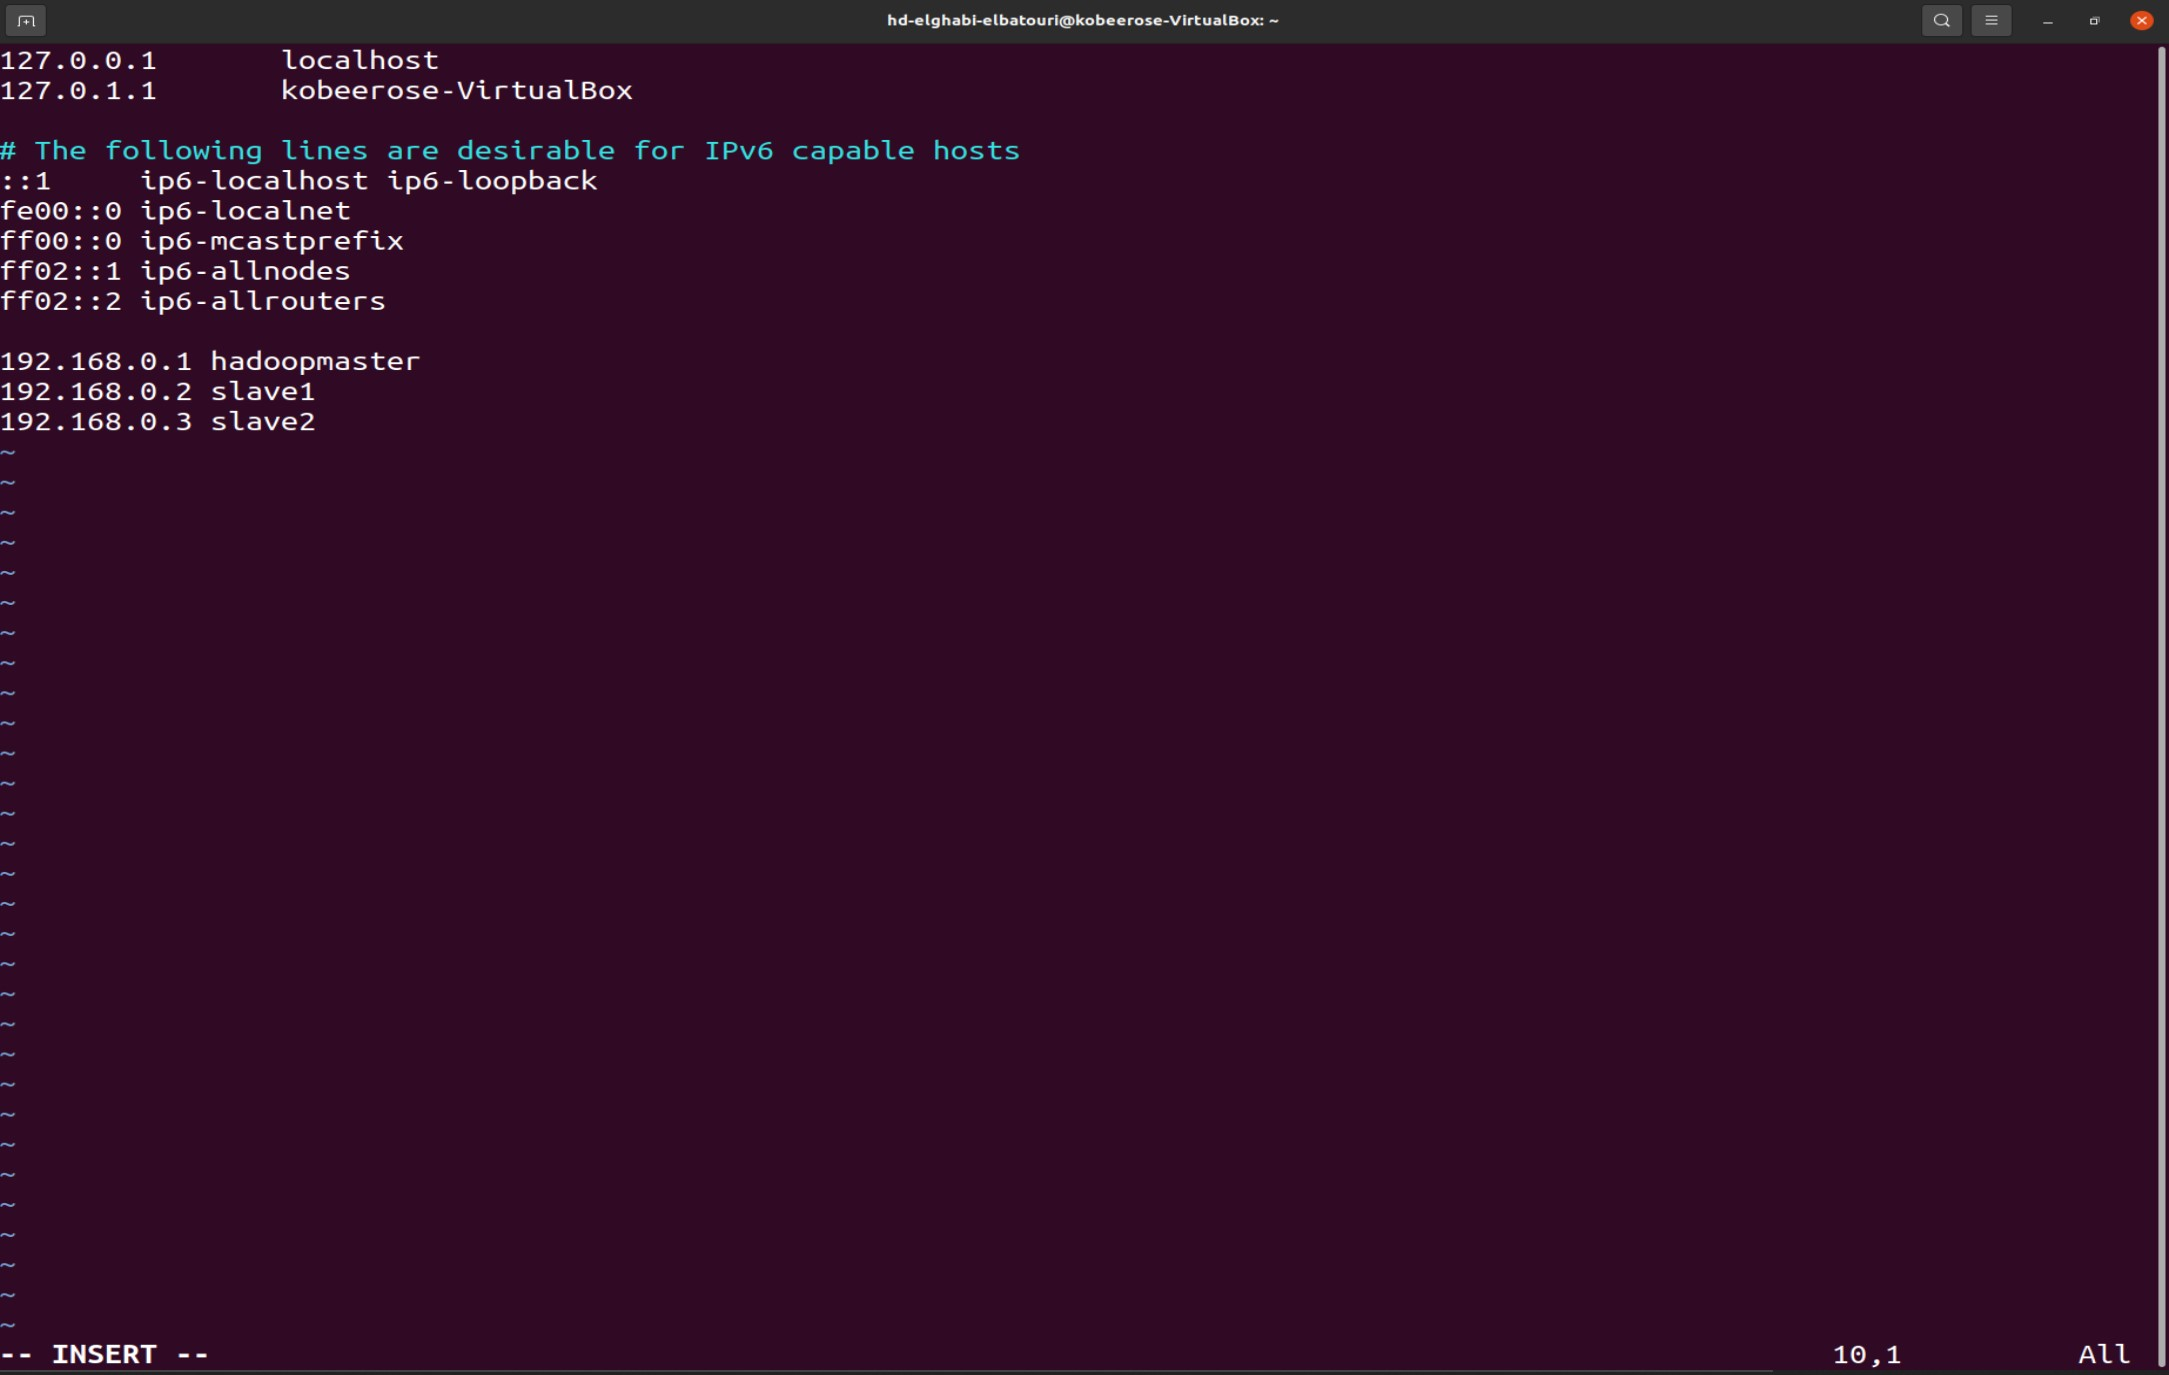
\includegraphics[width=1\linewidth]{Big_Data/Hadoop/Multi-Nodes Cluster/Adding Hosts.jpg} 
\end{center} 
\caption{caption} 
\end{figure} 
\FloatBarrier



\par we use to configure the IP address the "1-network-manager all.yaml" file found in the /etc/netplan/ directory.
\\
\begin{figure}[!htb] 
\begin{center} 
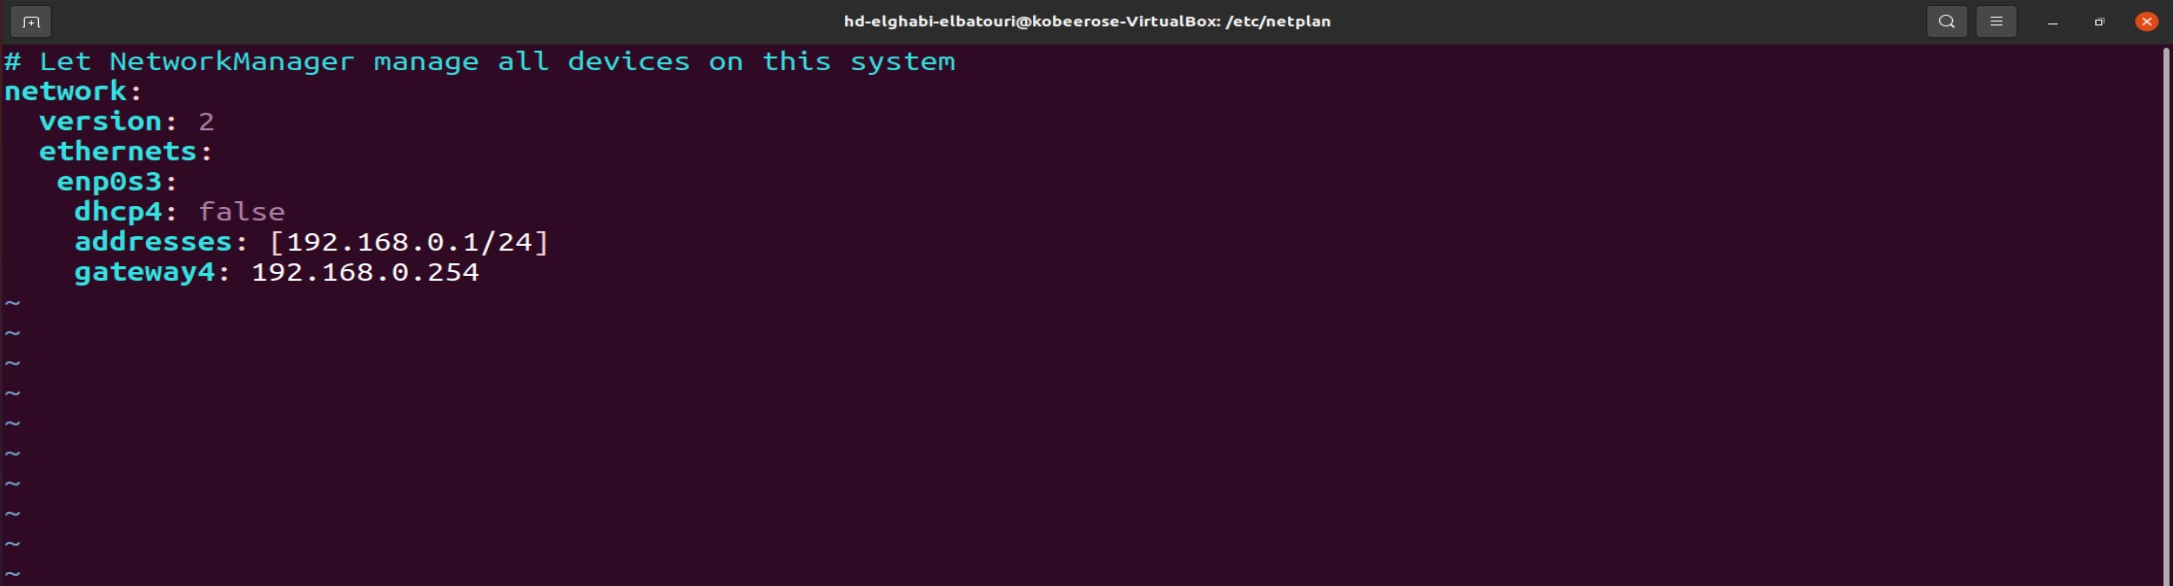
\includegraphics[width=1\linewidth]{Big_Data/Hadoop/Multi-Nodes Cluster/Fixing the IP adresse.jpg} 
\end{center} 
\caption{caption} 
\end{figure} 
\FloatBarrier

\section{Modification des fichiers de configuration de hadoop}

\par Editing Hadoop Configuration Files: core-site.xml, hdfs-site.xml, mapred-site.xml, yarn-site.xml. 
\\
\begin{figure}[!htb] 
\begin{center} 
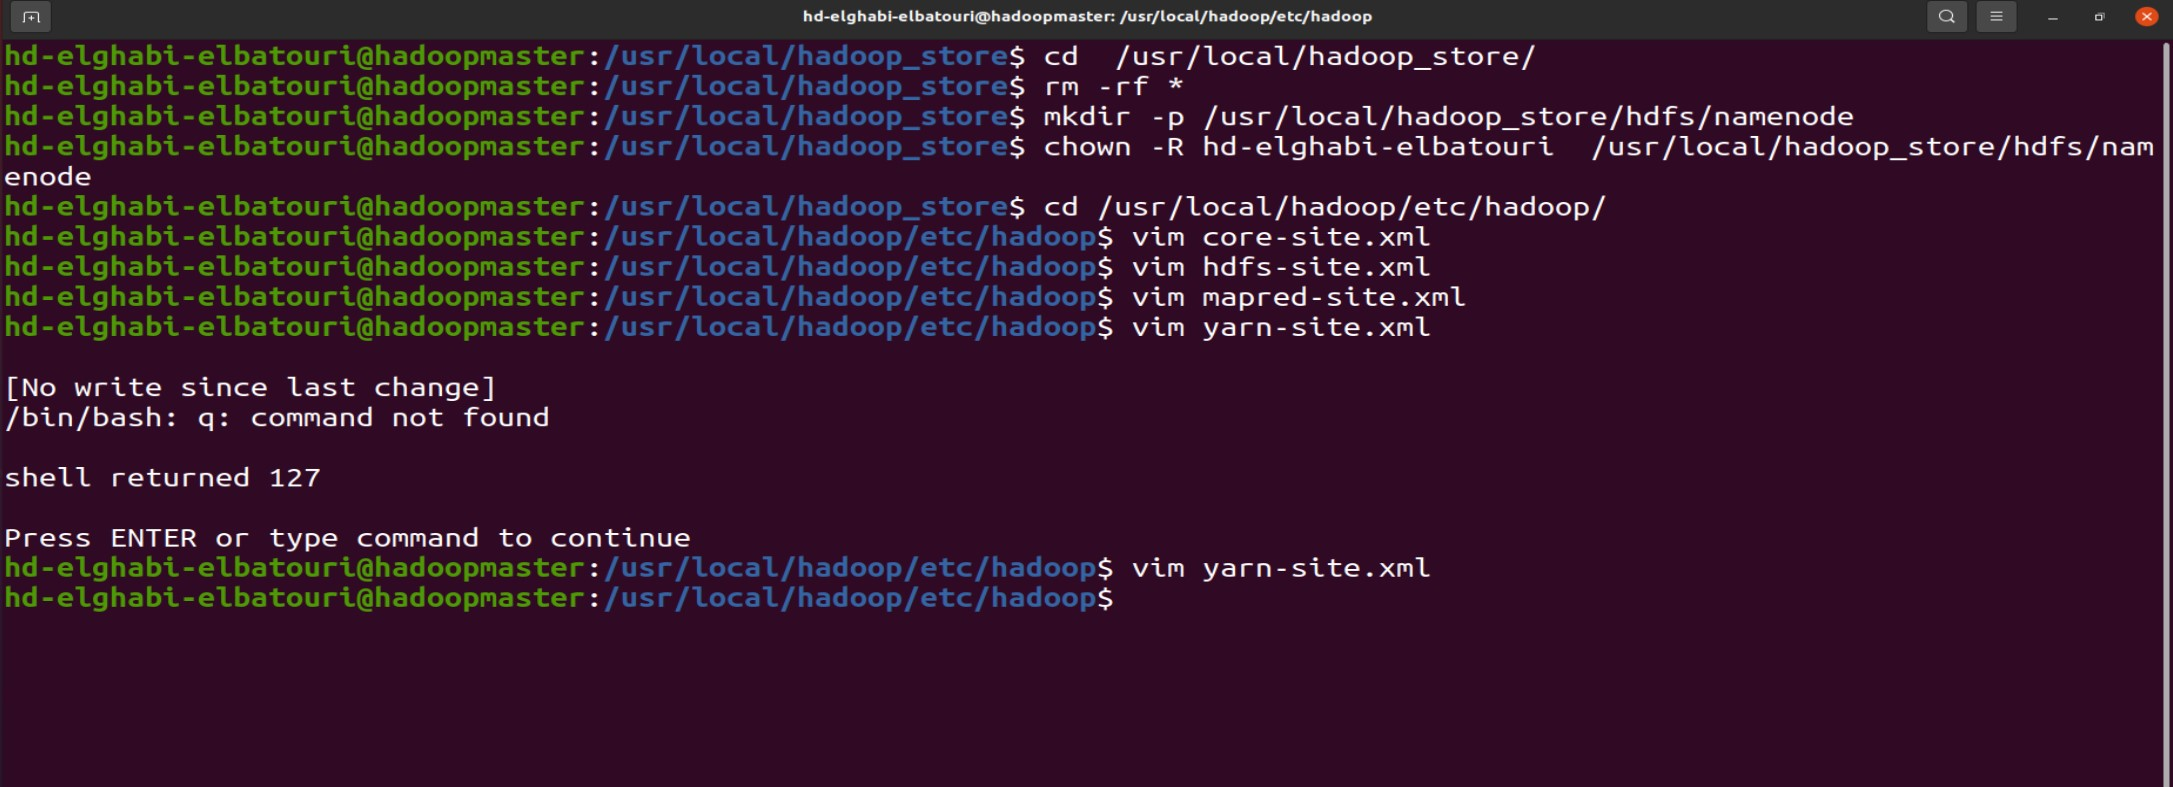
\includegraphics[width=1\linewidth]{Big_Data/Hadoop/Multi-Nodes Cluster/Modifying Hadoop config files.jpg} 
\end{center} 
\caption{caption} 
\end{figure} 
\FloatBarrier



\par Create the masters file which contains the hostname of the master machine, and the workers file which contains the hostname of each slave machine in the directory.
\\
\begin{figure}[!htb] 
\begin{center} 
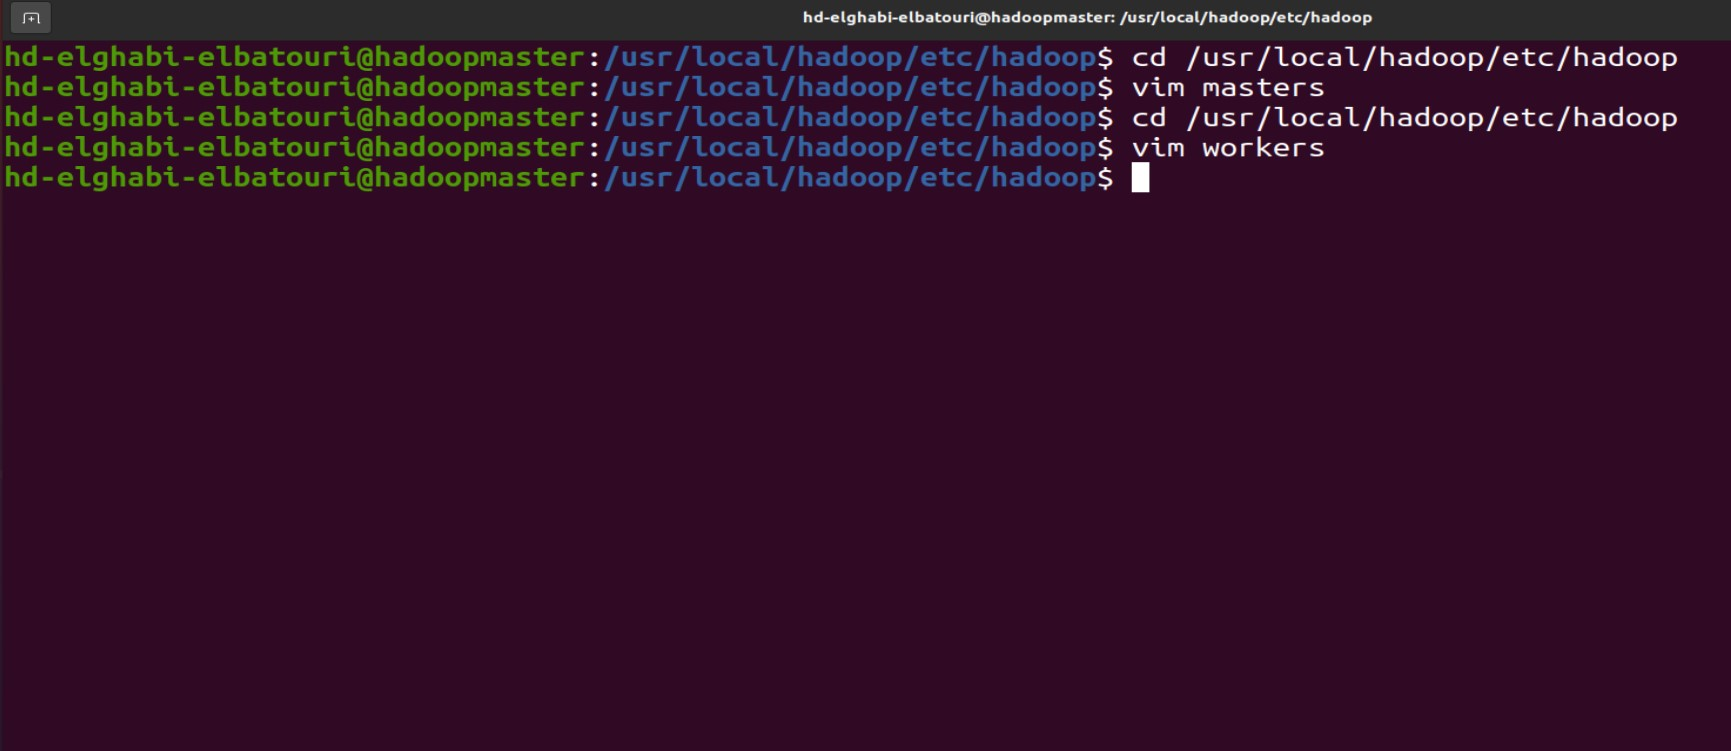
\includegraphics[width=1\linewidth]{Big_Data/Hadoop/Multi-Nodes Cluster/Master and Workers.jpg} 
\end{center} 
\caption{caption} 
\end{figure} 
\FloatBarrier

\section{Connection between cluster machines}

\par After cloning of the hadoop master machine and making the Modifications to be made in the slave1 and slave2 machines, we will test the connection between the machines.
\\
\begin{figure}[!htb] 
\begin{center} 
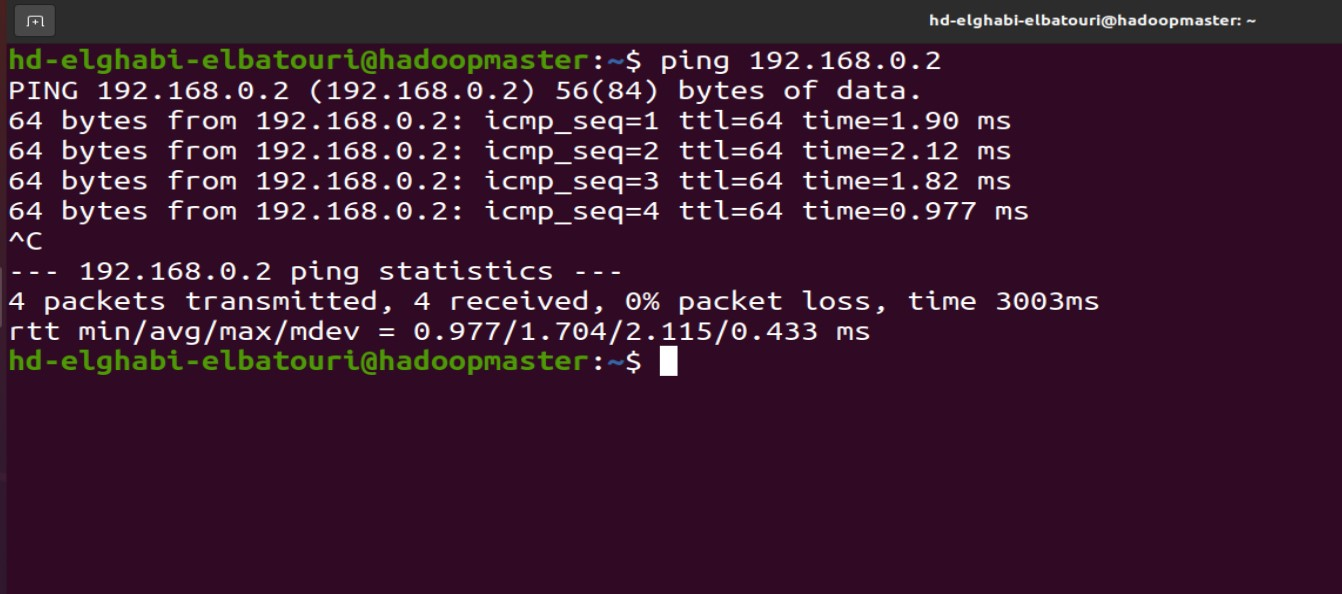
\includegraphics[width=1\linewidth]{Big_Data/Hadoop/Multi-Nodes Cluster/Master ping to Slave1.jpg} 
\end{center} 
\caption{caption} 
\end{figure} 
\FloatBarrier

\\
\begin{figure}[!htb] 
\begin{center} 
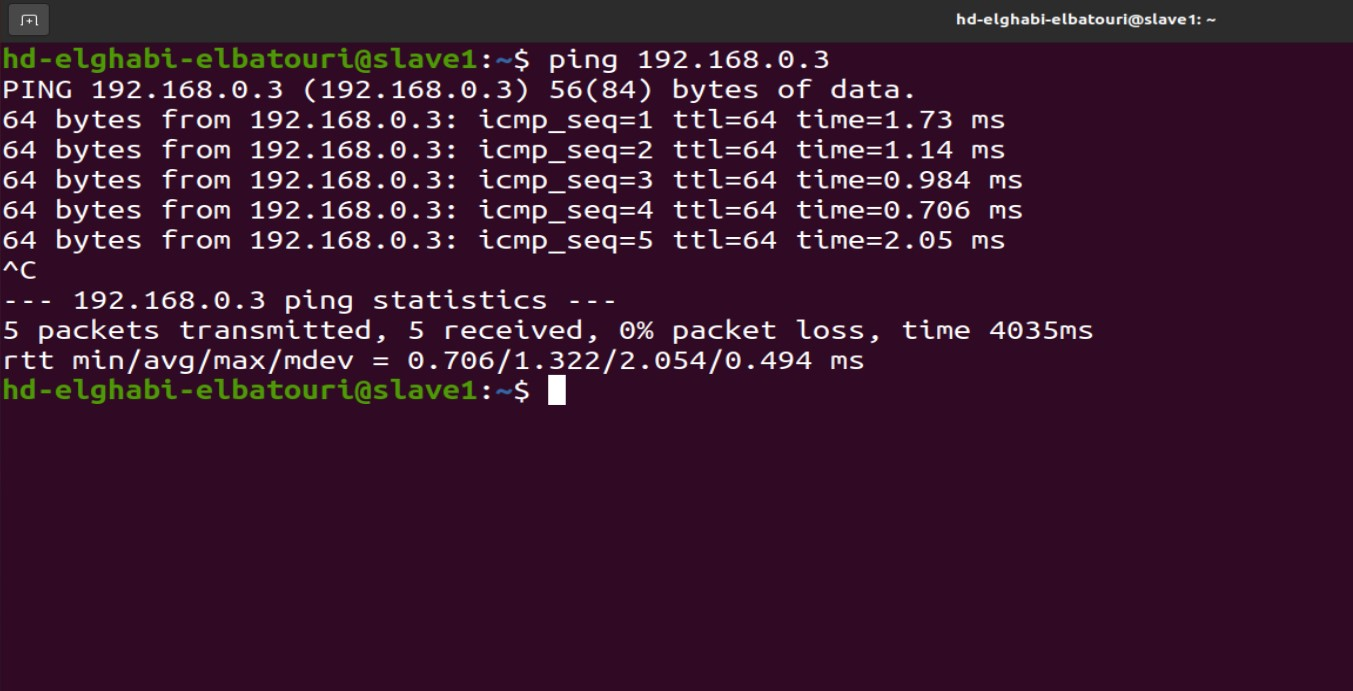
\includegraphics[width=1\linewidth]{Big_Data/Hadoop/Multi-Nodes Cluster/Slave1 ping to Slave2.jpg} 
\end{center} 
\caption{caption} 
\end{figure} 
\FloatBarrier
\\
\begin{figure}[!htb] 
\begin{center} 
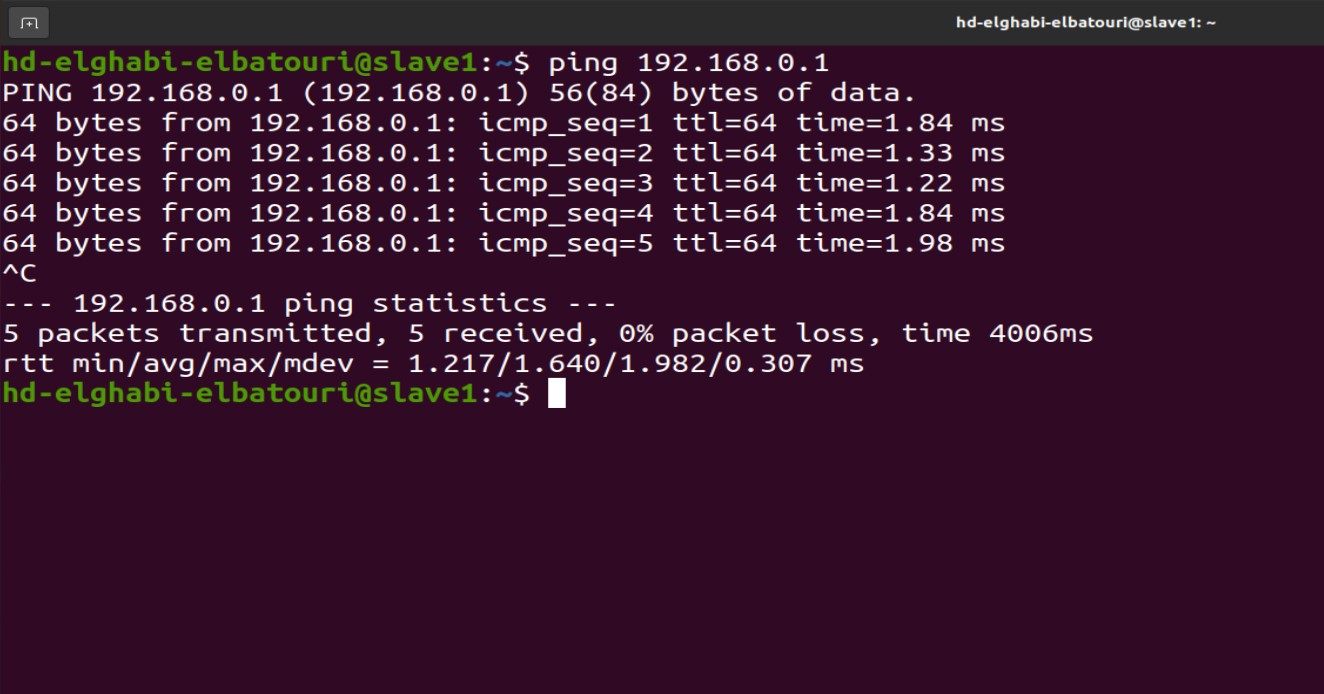
\includegraphics[width=1\linewidth]{Big_Data/Hadoop/Multi-Nodes Cluster/Slave2 ping to Master.jpg} 
\end{center} 
\caption{caption} 
\end{figure} 
\FloatBarrier

\par Copying the ssh key to configure passwordless ssh access between machines in the cluster.
\\
\begin{figure}[!htb] 
\begin{center} 
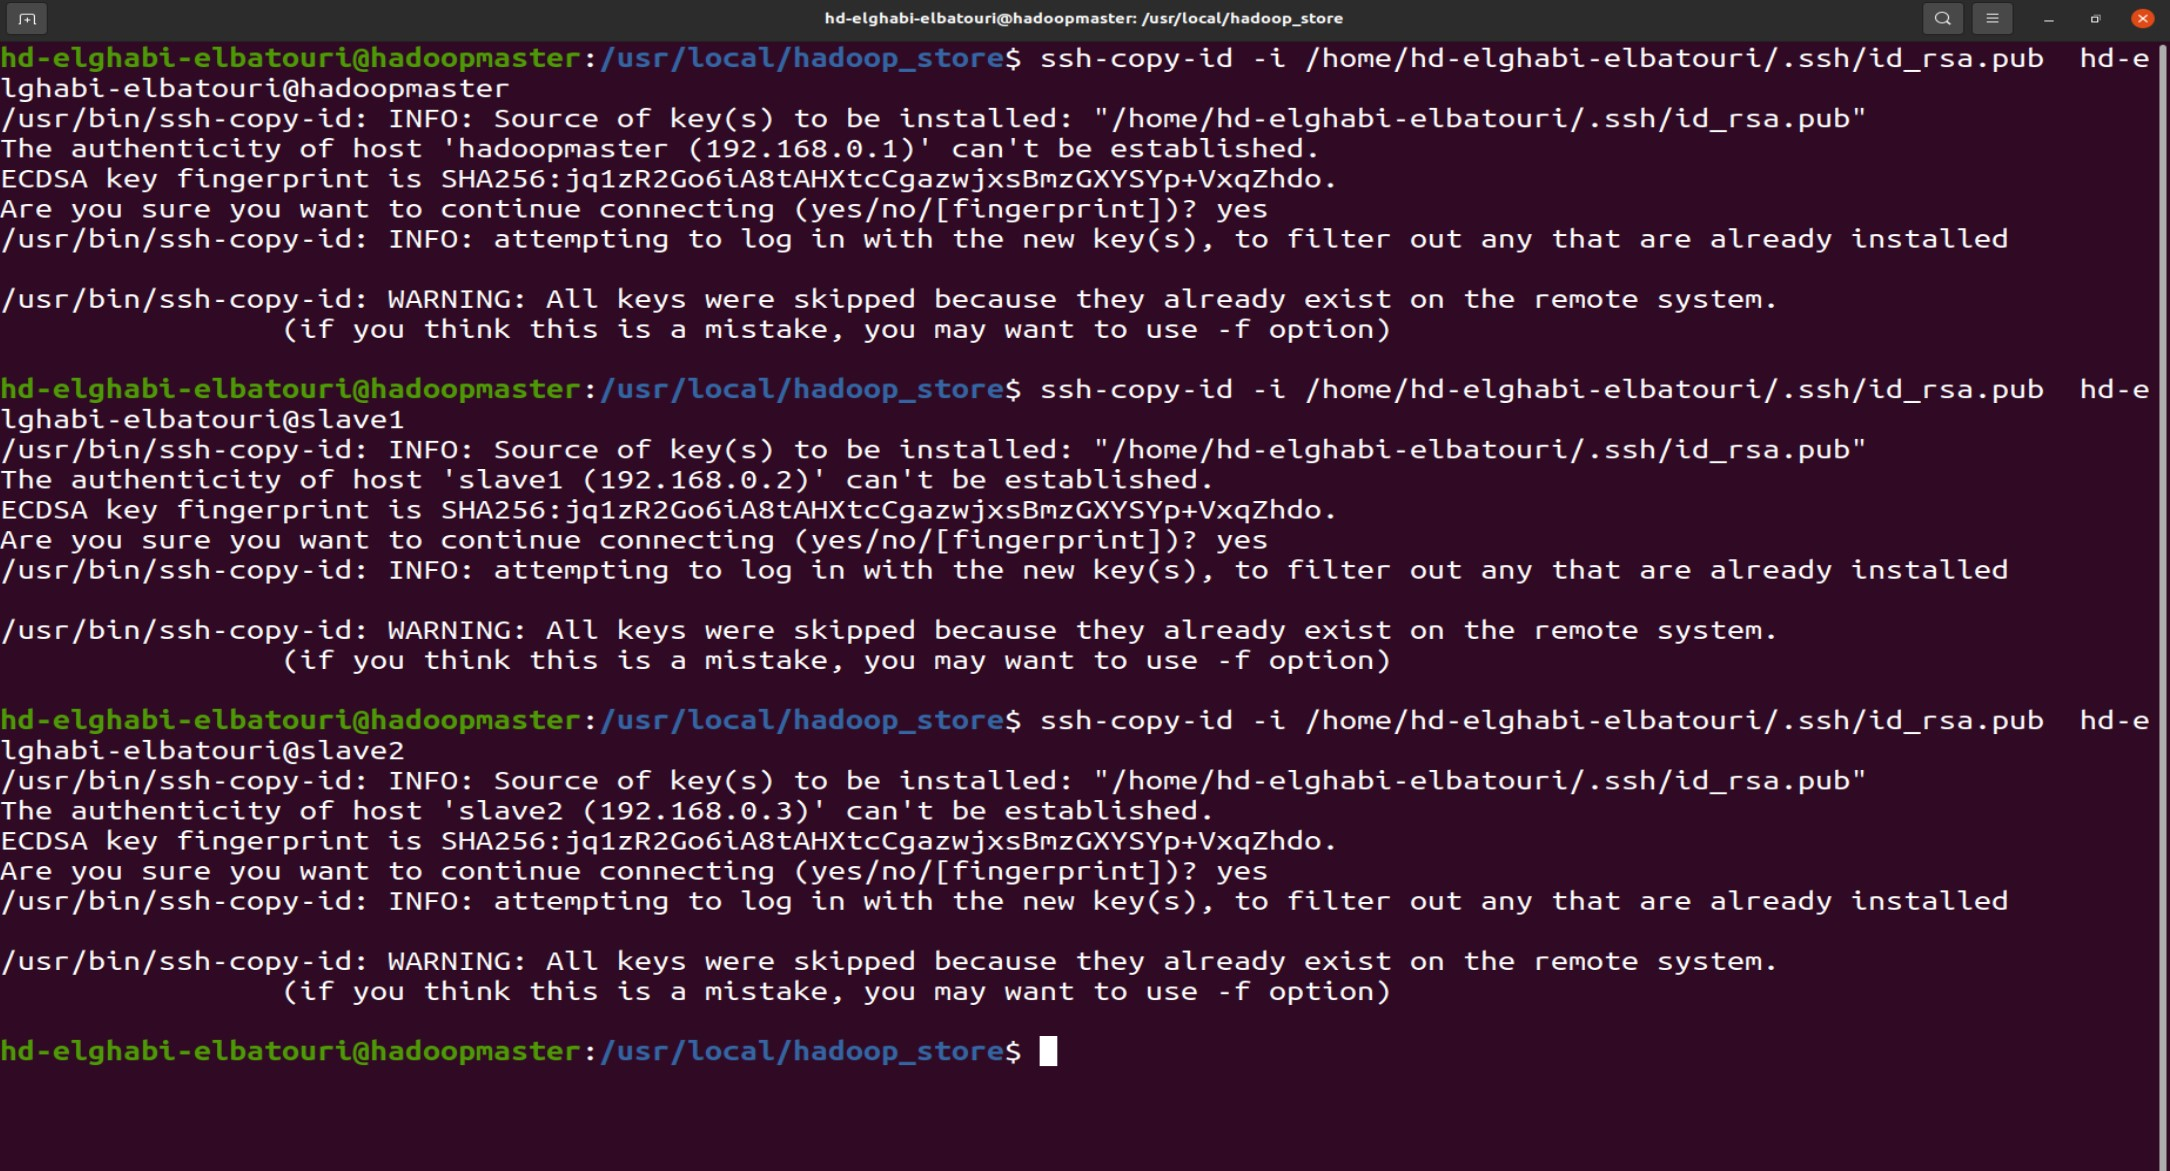
\includegraphics[width=1\linewidth]{Big_Data/Hadoop/Multi-Nodes Cluster/ssh key between machines.jpg} 
\end{center} 
\caption{caption} 
\end{figure} 
\FloatBarrier



\par Trying ssh between all the machines.
\\
\begin{figure}[!htb] 
\begin{center} 
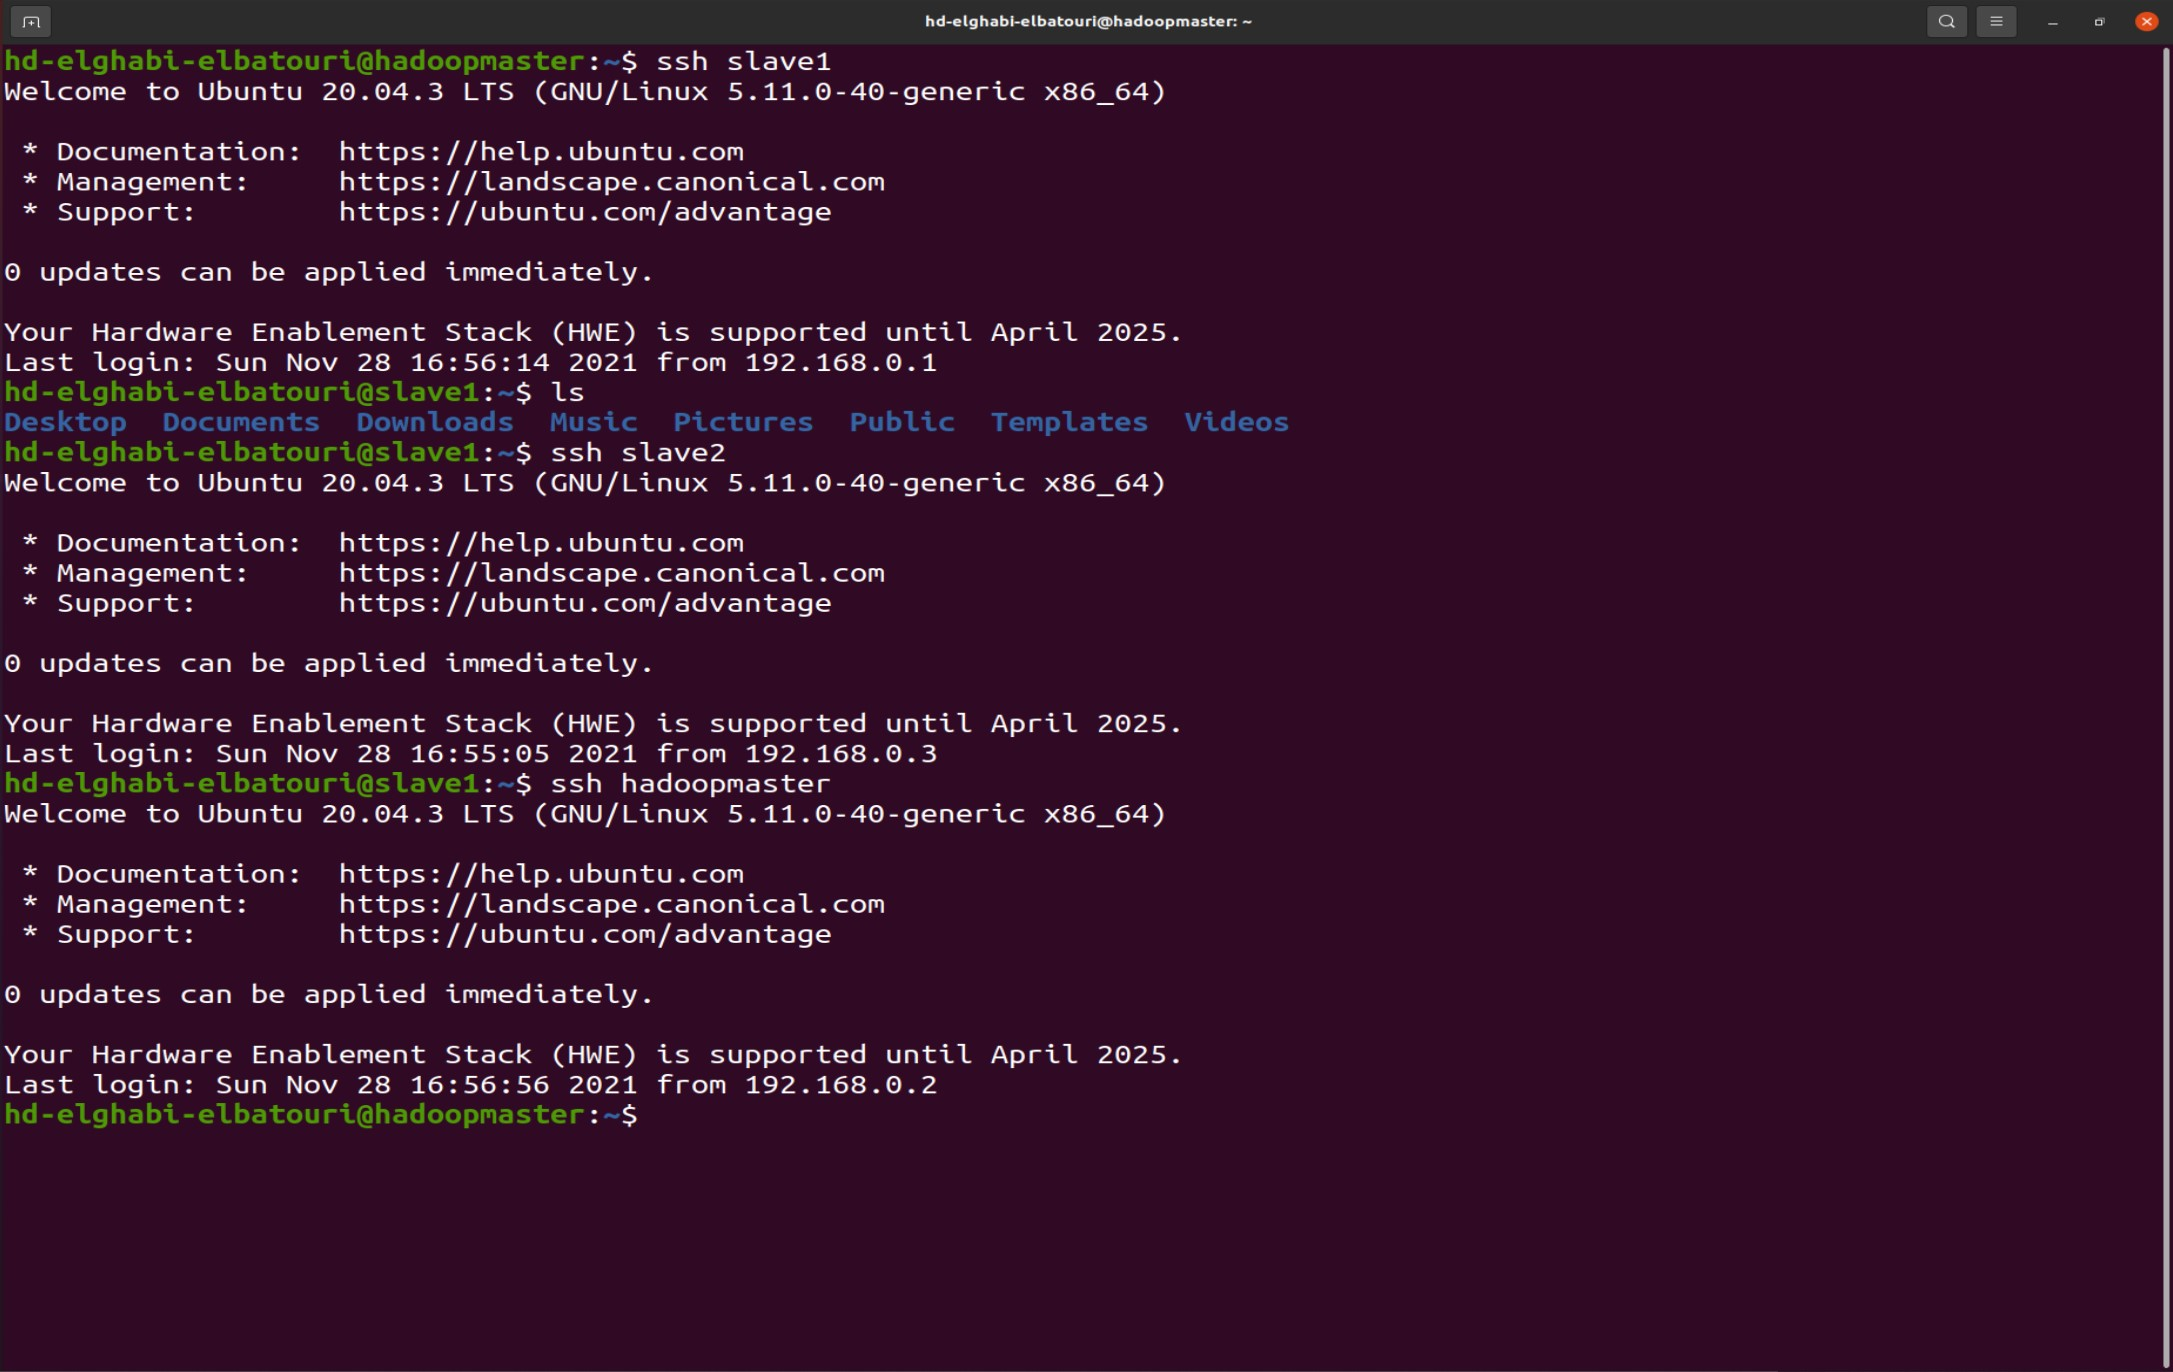
\includegraphics[width=1\linewidth]{Big_Data/Hadoop/Multi-Nodes Cluster/sshing between machines.jpg} 
\end{center} 
\caption{caption} 
\end{figure} 
\FloatBarrier

\section{Modifying hdfs config for slaves}

\par thisIsAveryLongParagraphToUseAsAtemplateForCopyAndPastingContentInAgoodWay
\\
\begin{figure}[!htb] 
\begin{center} 
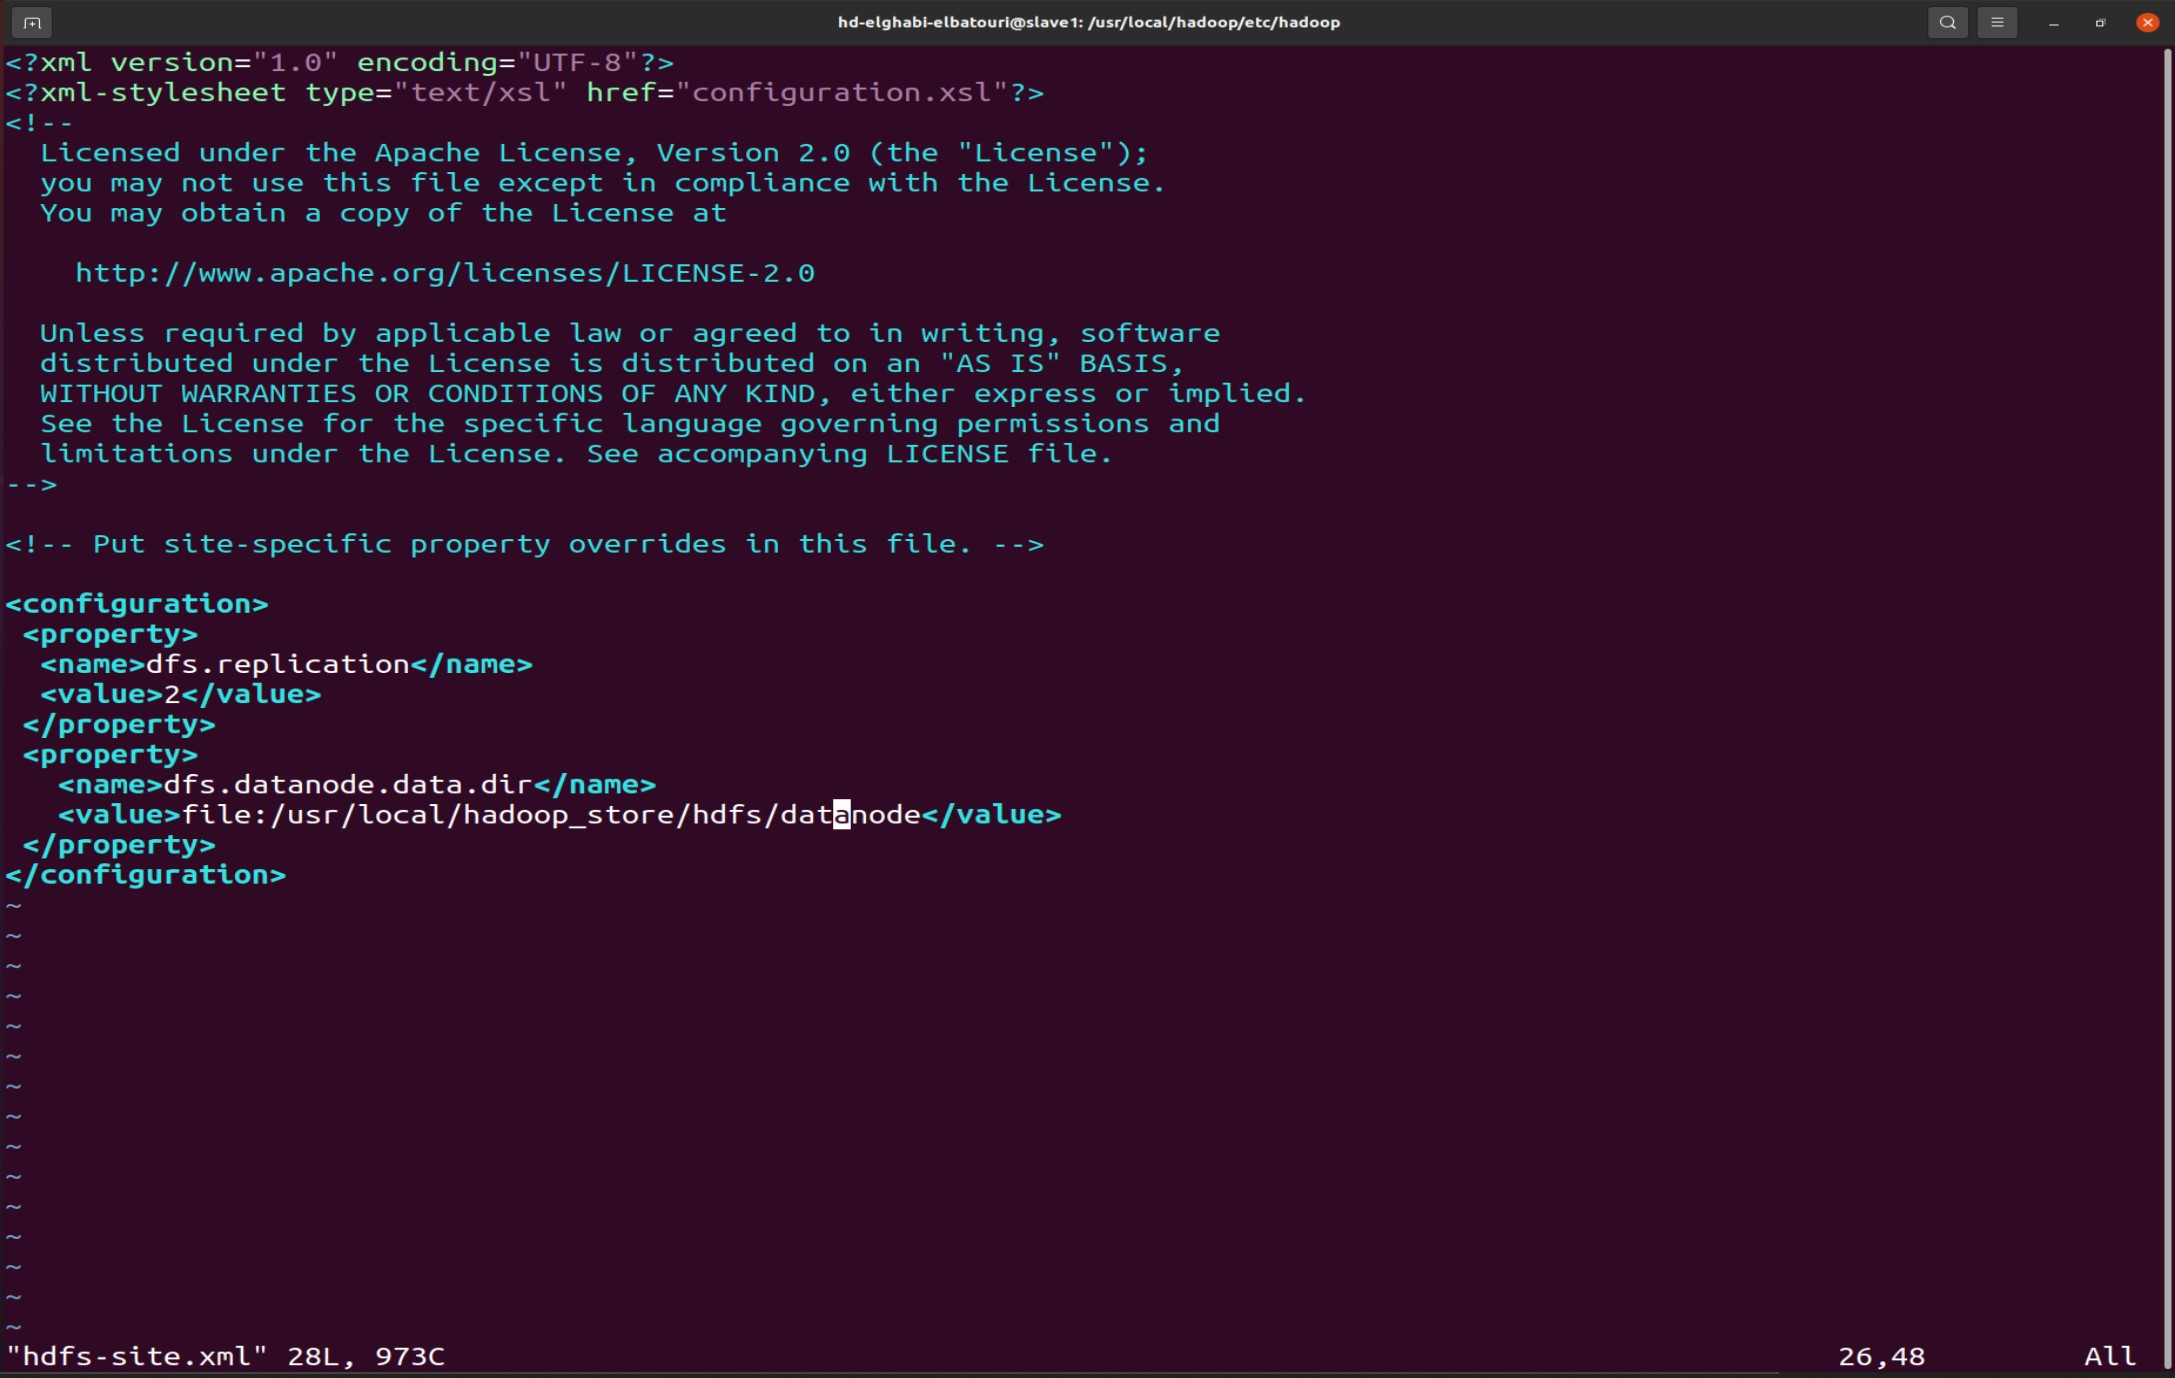
\includegraphics[width=1\linewidth]{Big_Data/Hadoop/Multi-Nodes Cluster/Modifying hdfs config for slaves.jpg} 
\end{center} 
\caption{caption} 
\end{figure} 
\FloatBarrier

\par it is also necessary to empty the storage directory of the node hadoopmaster and to re-format the hdfs namenode.
\\
\begin{figure}[!htb] 
\begin{center} 
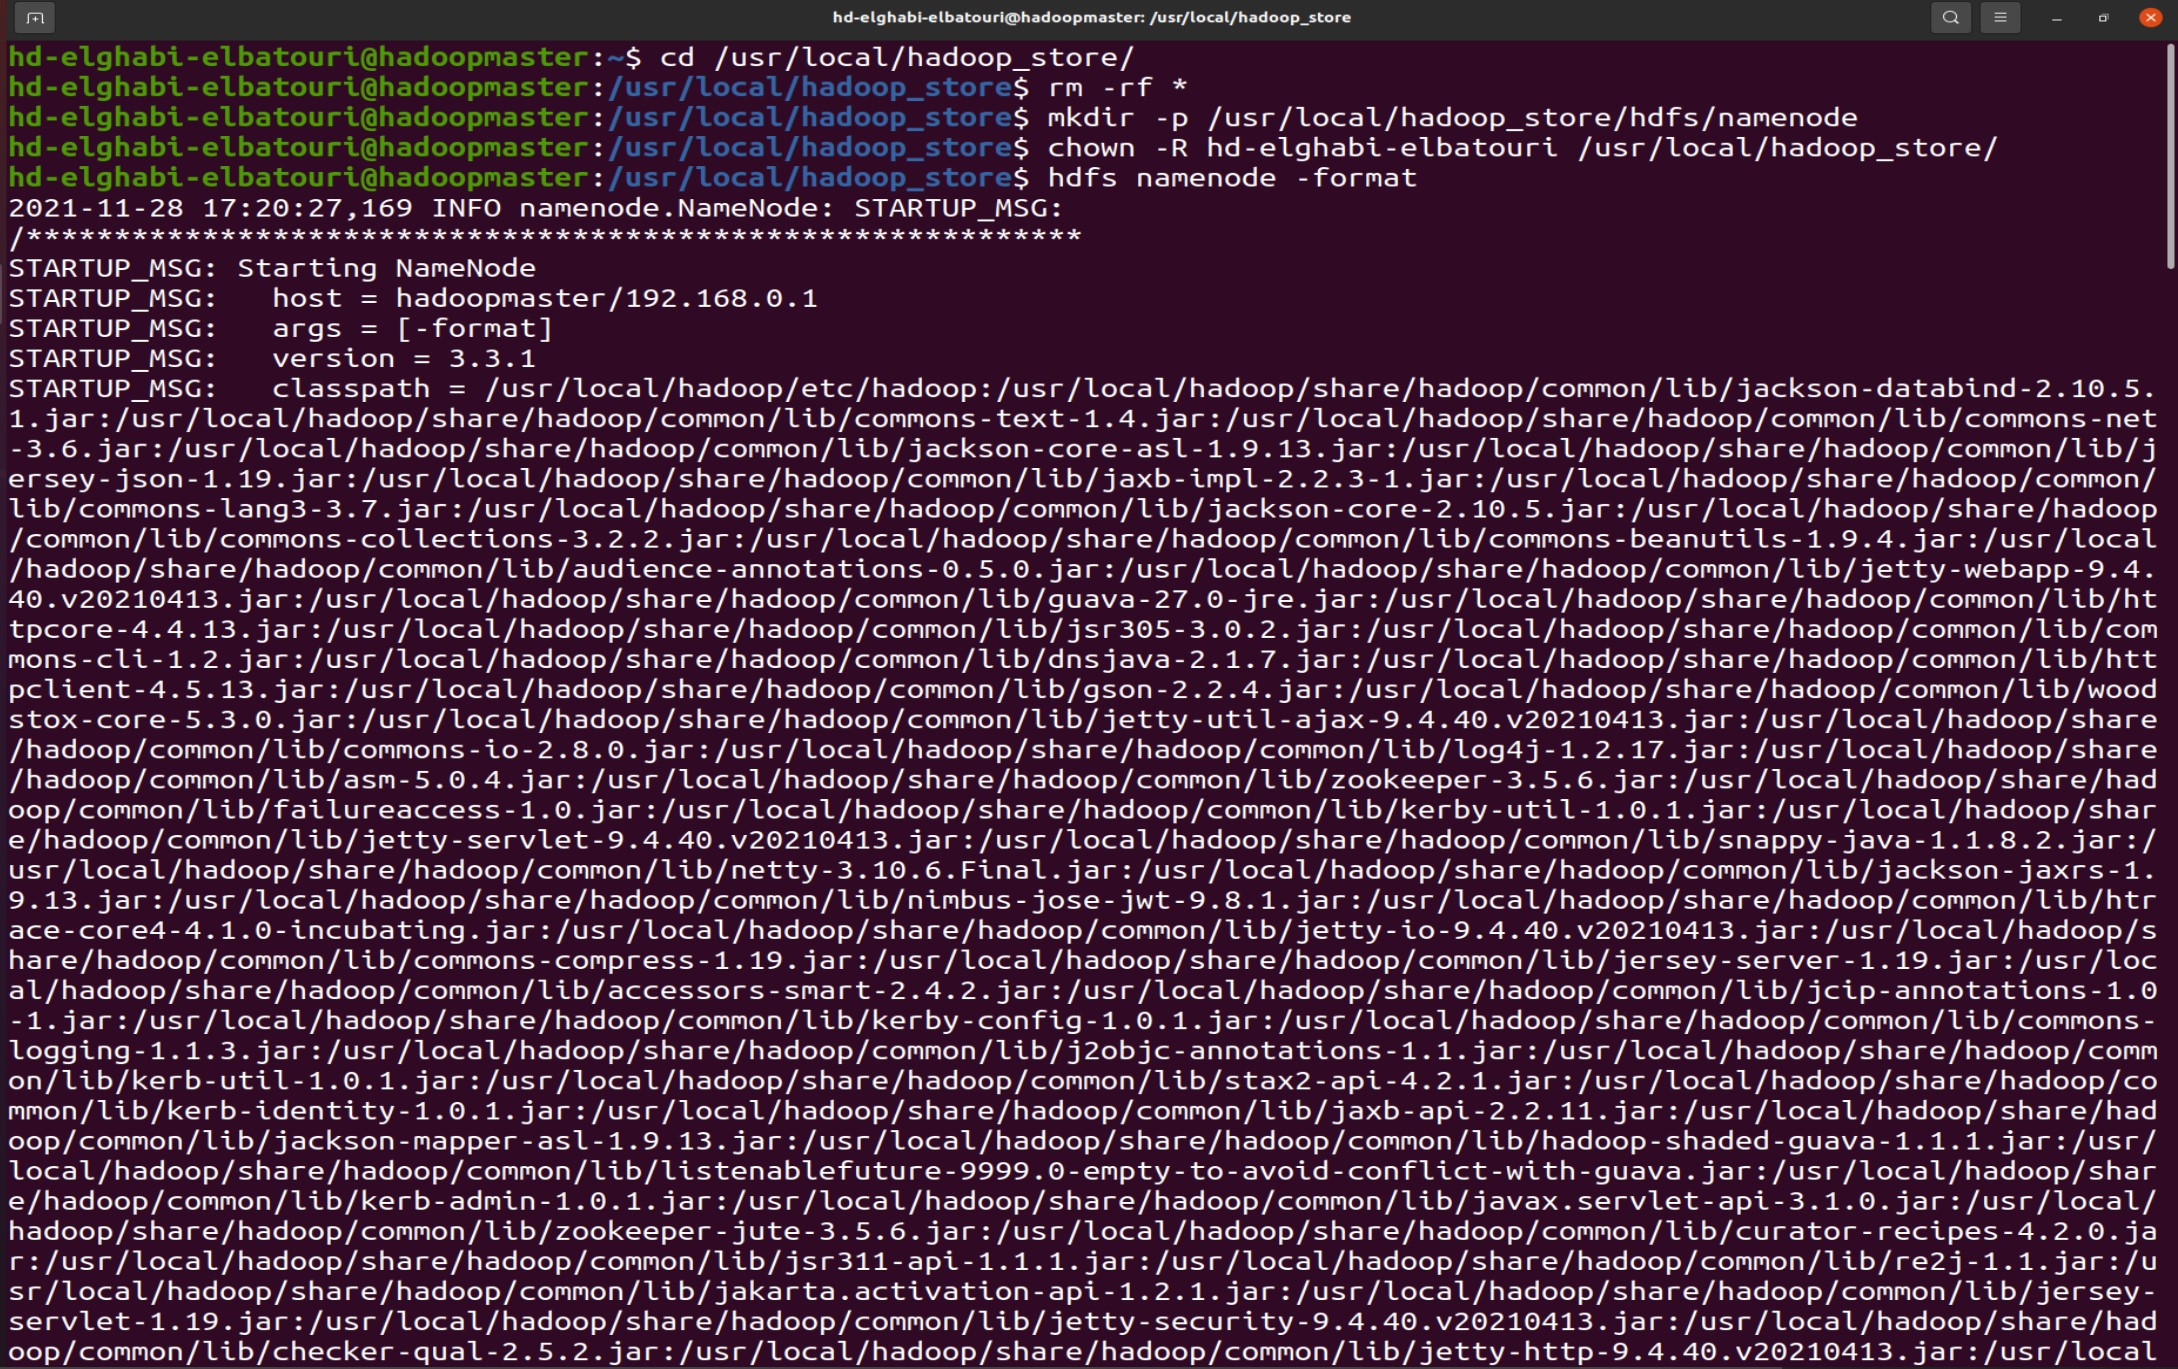
\includegraphics[width=1\linewidth]{Big_Data/Hadoop/Multi-Nodes Cluster/Formatting hadoopmaster namenode.jpg} 
\end{center} 
\caption{caption} 
\end{figure} 
\FloatBarrier


\par Starting the dfs and yarn and and running jps in each machine of the cluster.
\\
\begin{figure}[!htb] 
\begin{center} 
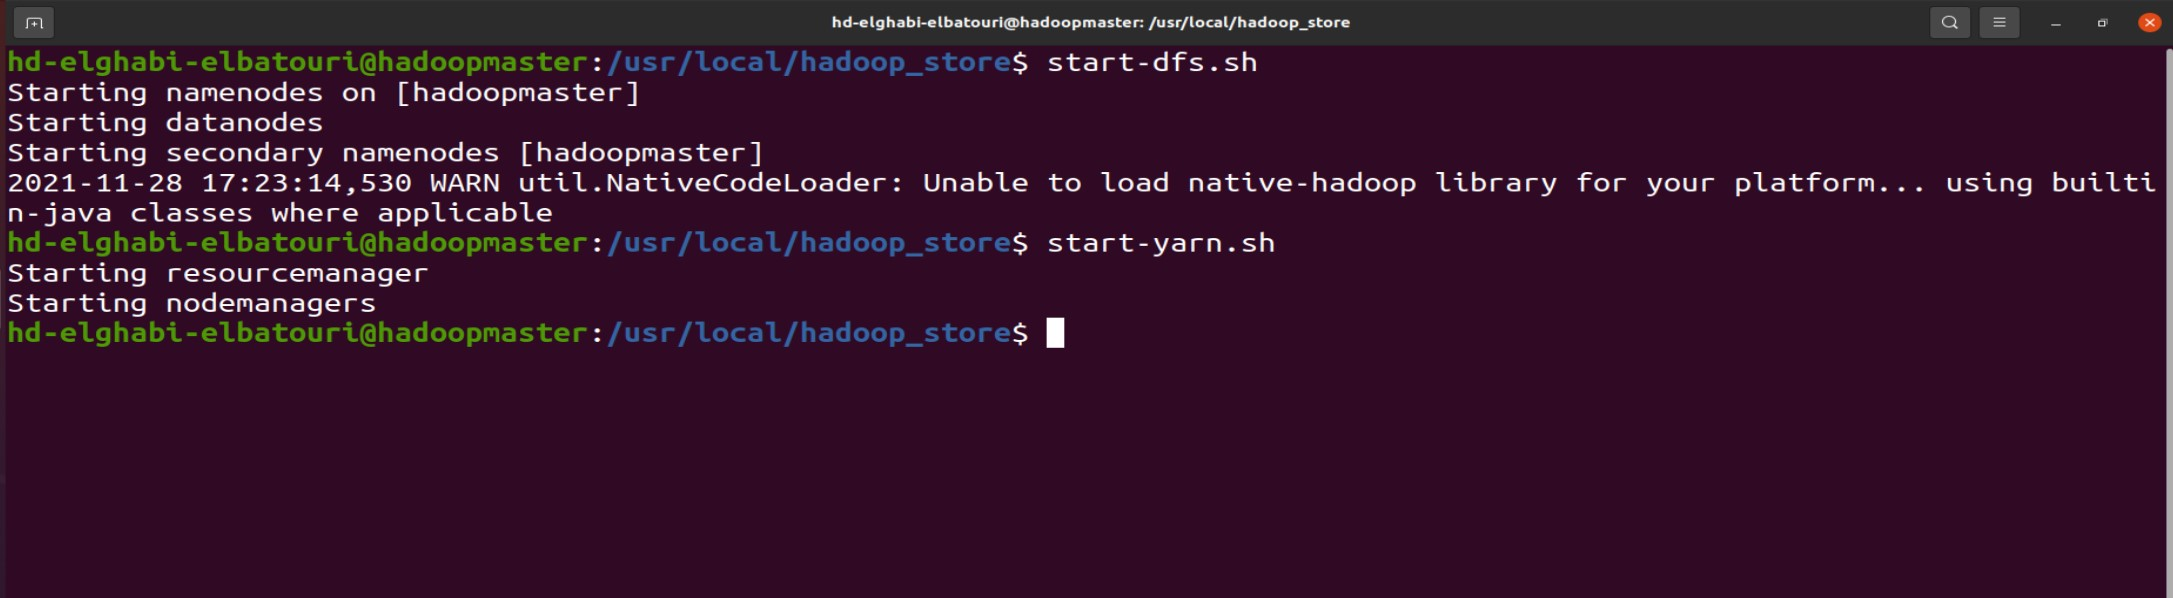
\includegraphics[width=1\linewidth]{Big_Data/Hadoop/Multi-Nodes Cluster/Starting dfs and yarn.jpg} 
\end{center} 
\caption{caption} 
\end{figure} 
\FloatBarrier


\section{Access Hadoop services through the browser}

\par Checking live nodes by navigating to http://hadoopmaster:9870/ on our web browser: 
\\
\begin{figure}[!htb] 
\begin{center} 
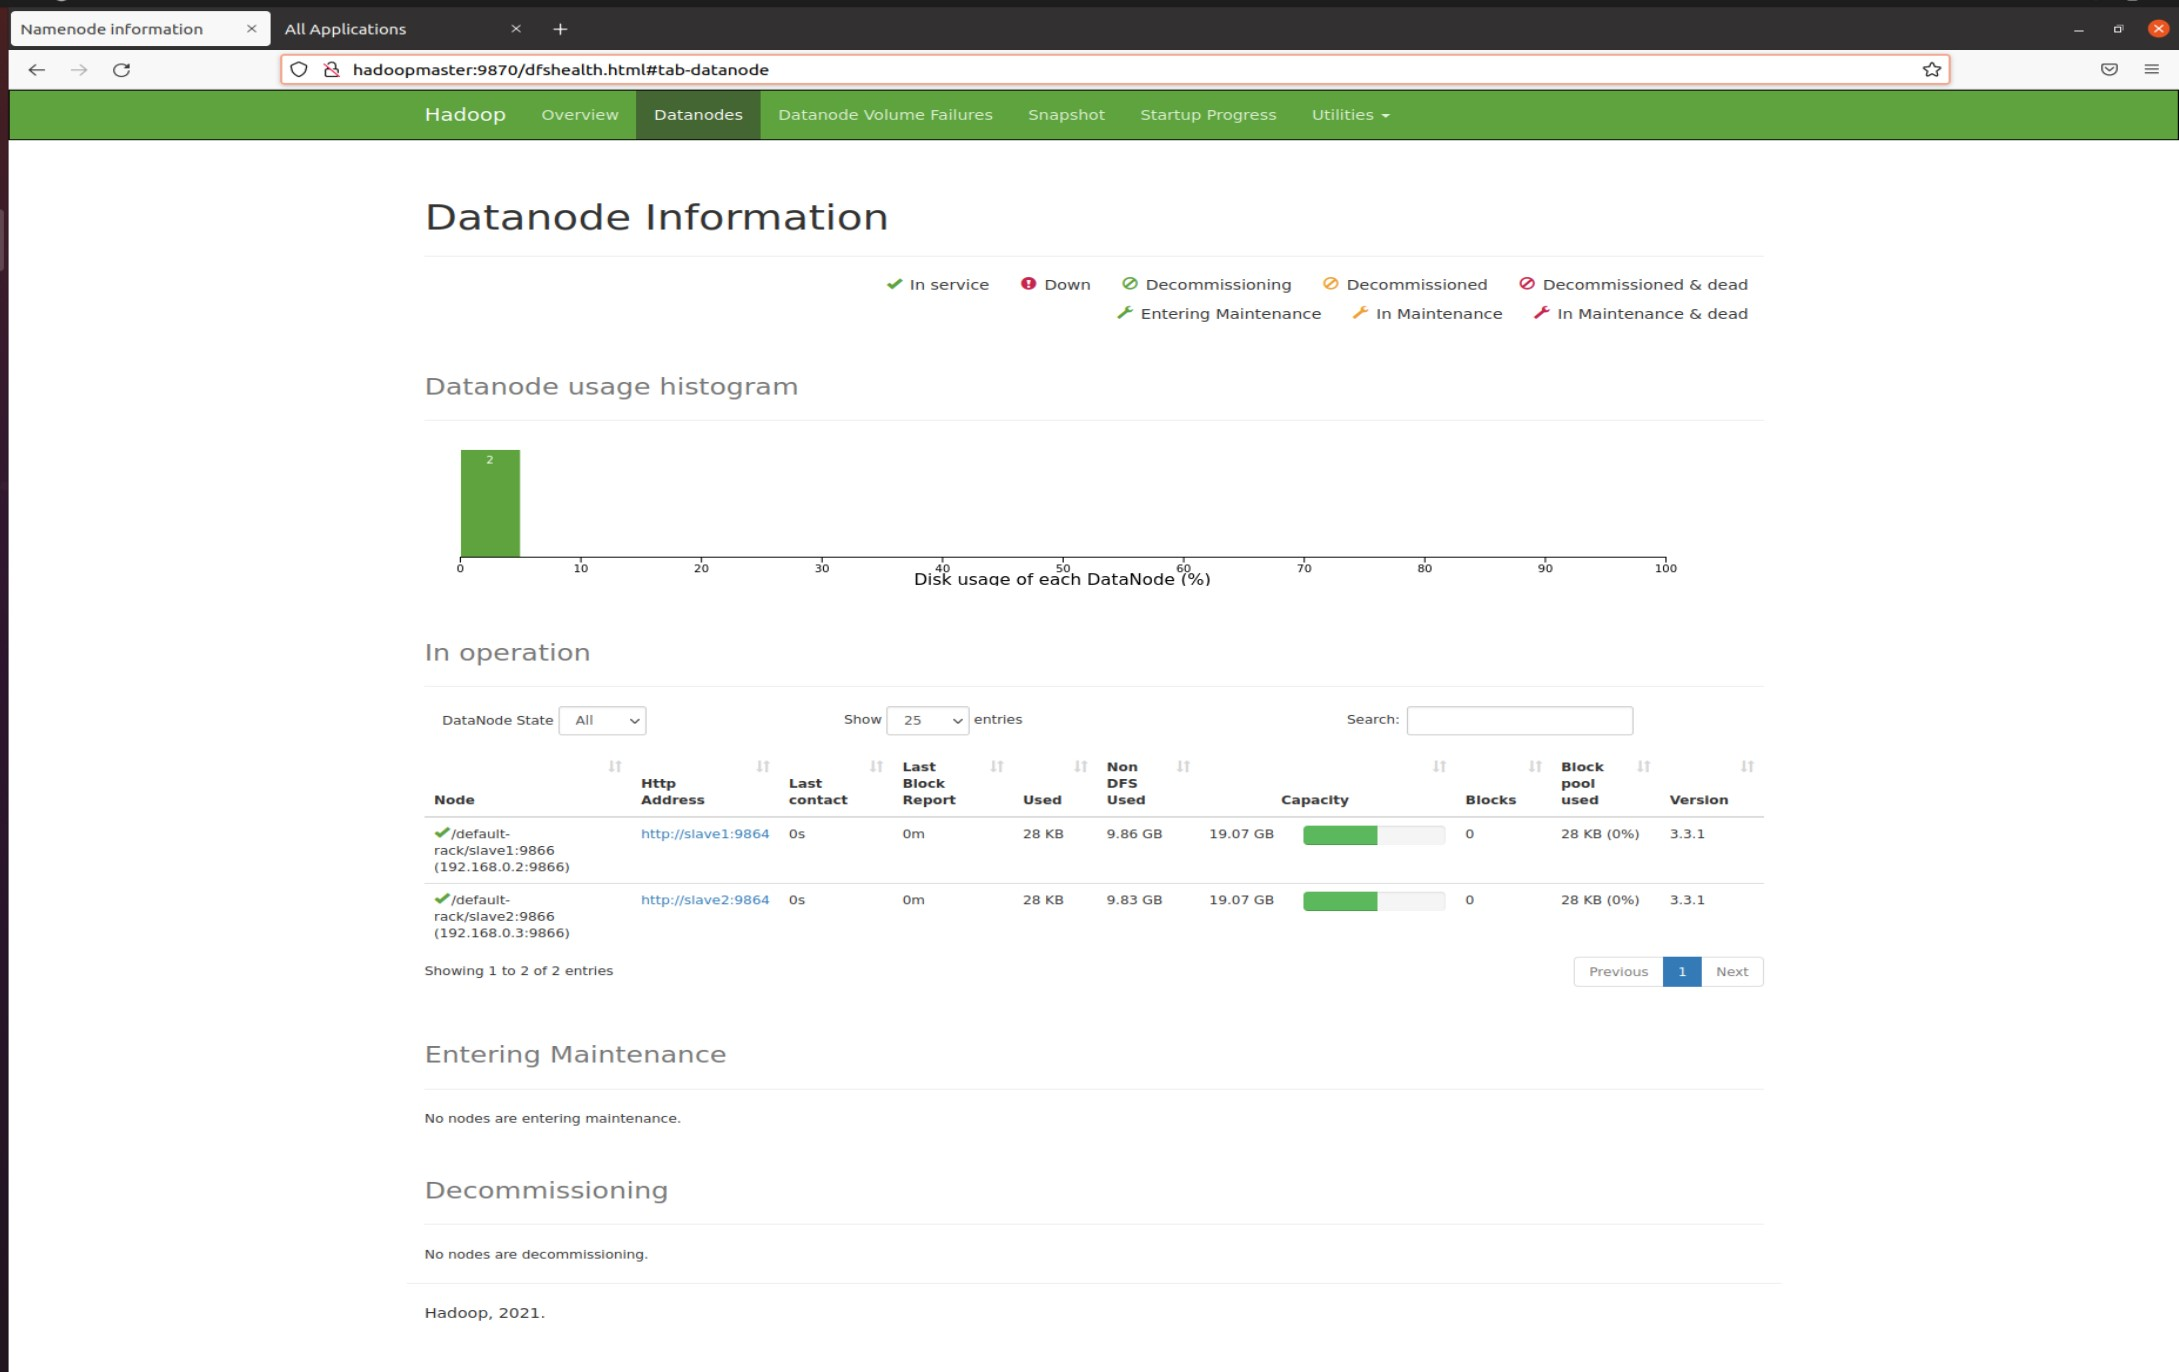
\includegraphics[width=1\linewidth]{Big_Data/Hadoop/Multi-Nodes Cluster/Checking live nodes.jpg} 
\end{center} 
\caption{caption} 
\end{figure} 
\FloatBarrier


\par Accessing the Resource manager interface on http://hadoopmaster:8088/
\\
\begin{figure}[!htb] 
\begin{center} 
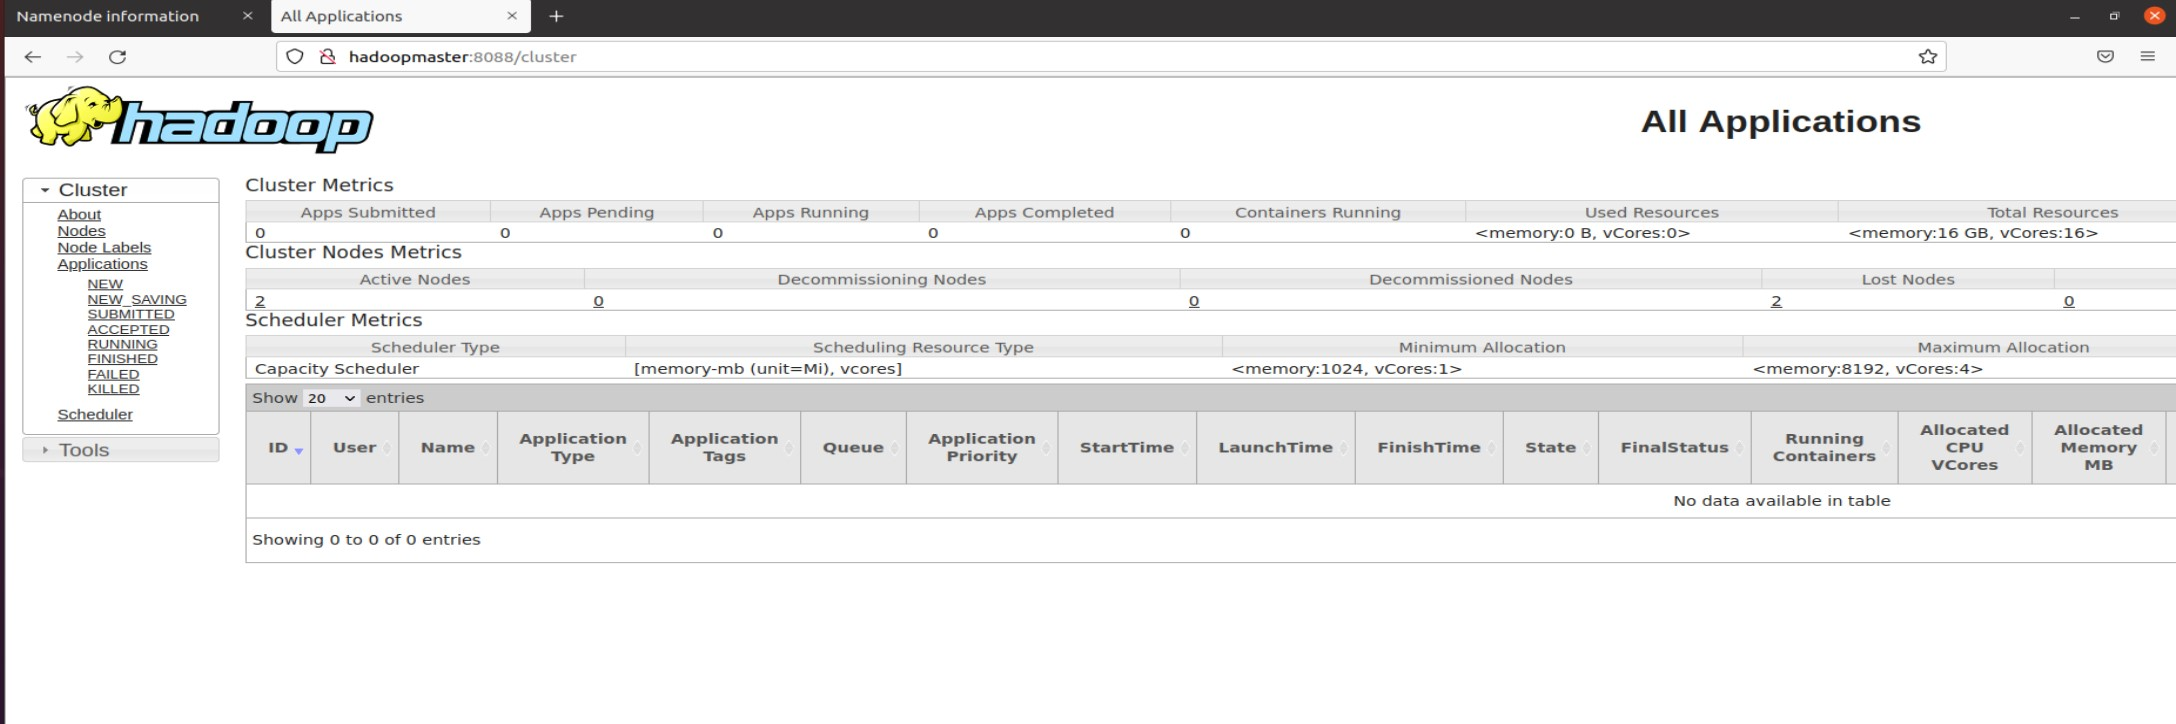
\includegraphics[width=1\linewidth]{Big_Data/Hadoop/Multi-Nodes Cluster/Ressource manager interface.jpg} 
\end{center} 
\caption{caption} 
\end{figure} 
\FloatBarrier

\section{Adding the hadoopmaster node as a datanode }

\par Editing the hdfs-site.xml file of hadoopmaster.
\\
\begin{figure}[!htb] 
\begin{center} 
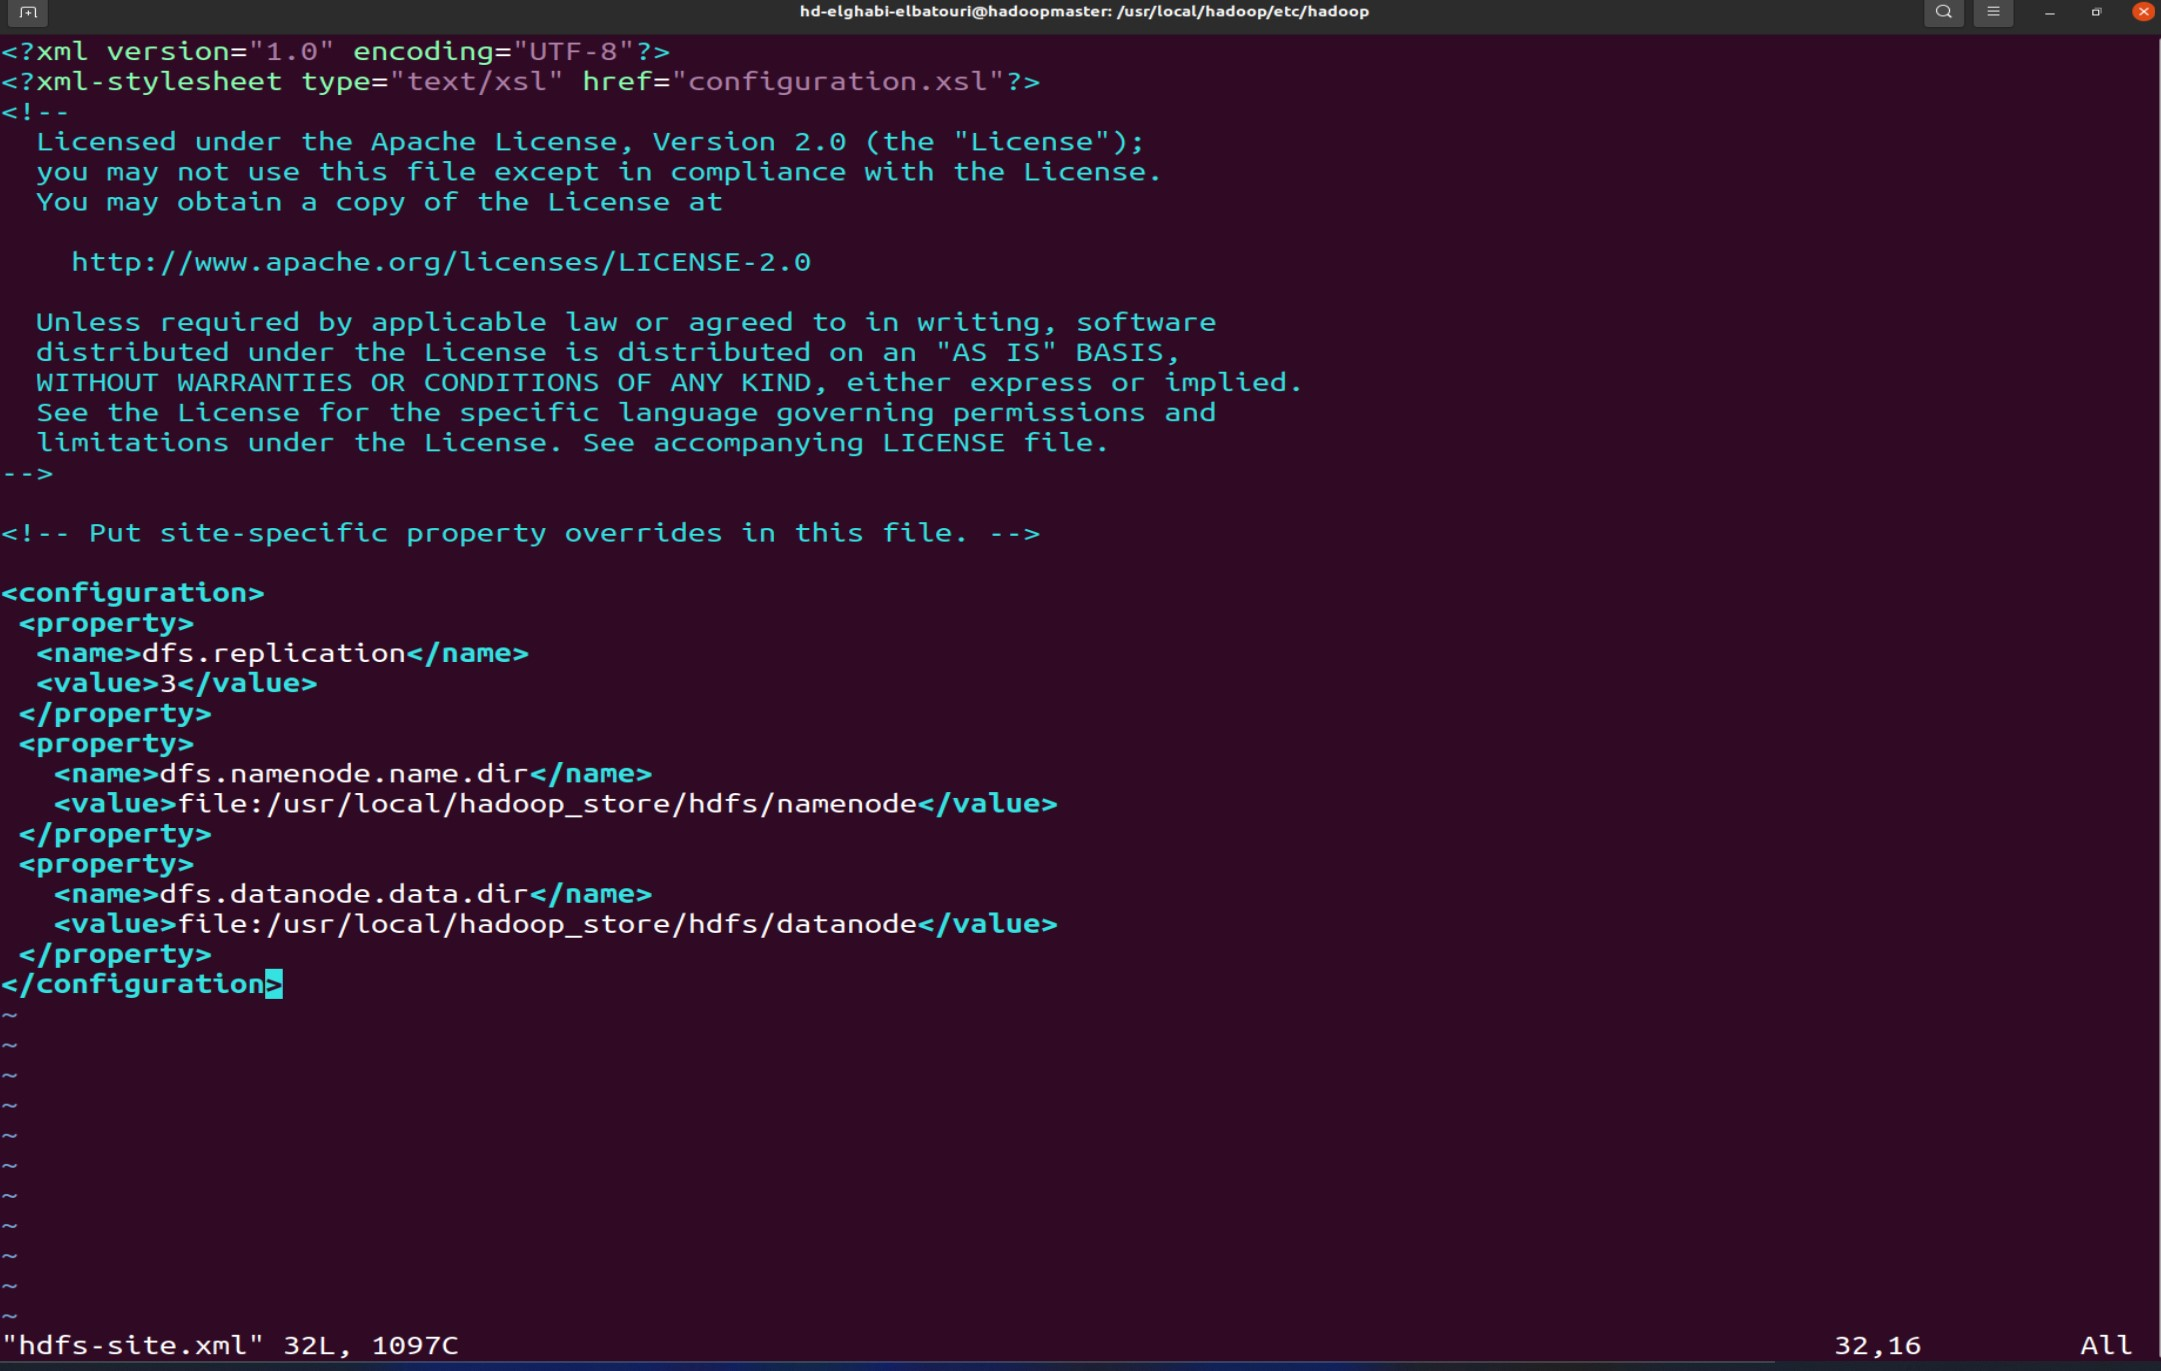
\includegraphics[width=1\linewidth]{Big_Data/Hadoop/Multi-Nodes Cluster/adding hadoopmaster as datanode.jpg} 
\end{center} 
\caption{caption} 
\end{figure} 
\FloatBarrier


\par Editing the hdfs-site.xml file for slave1 and slave2.
\\
\begin{figure}[!htb] 
\begin{center} 
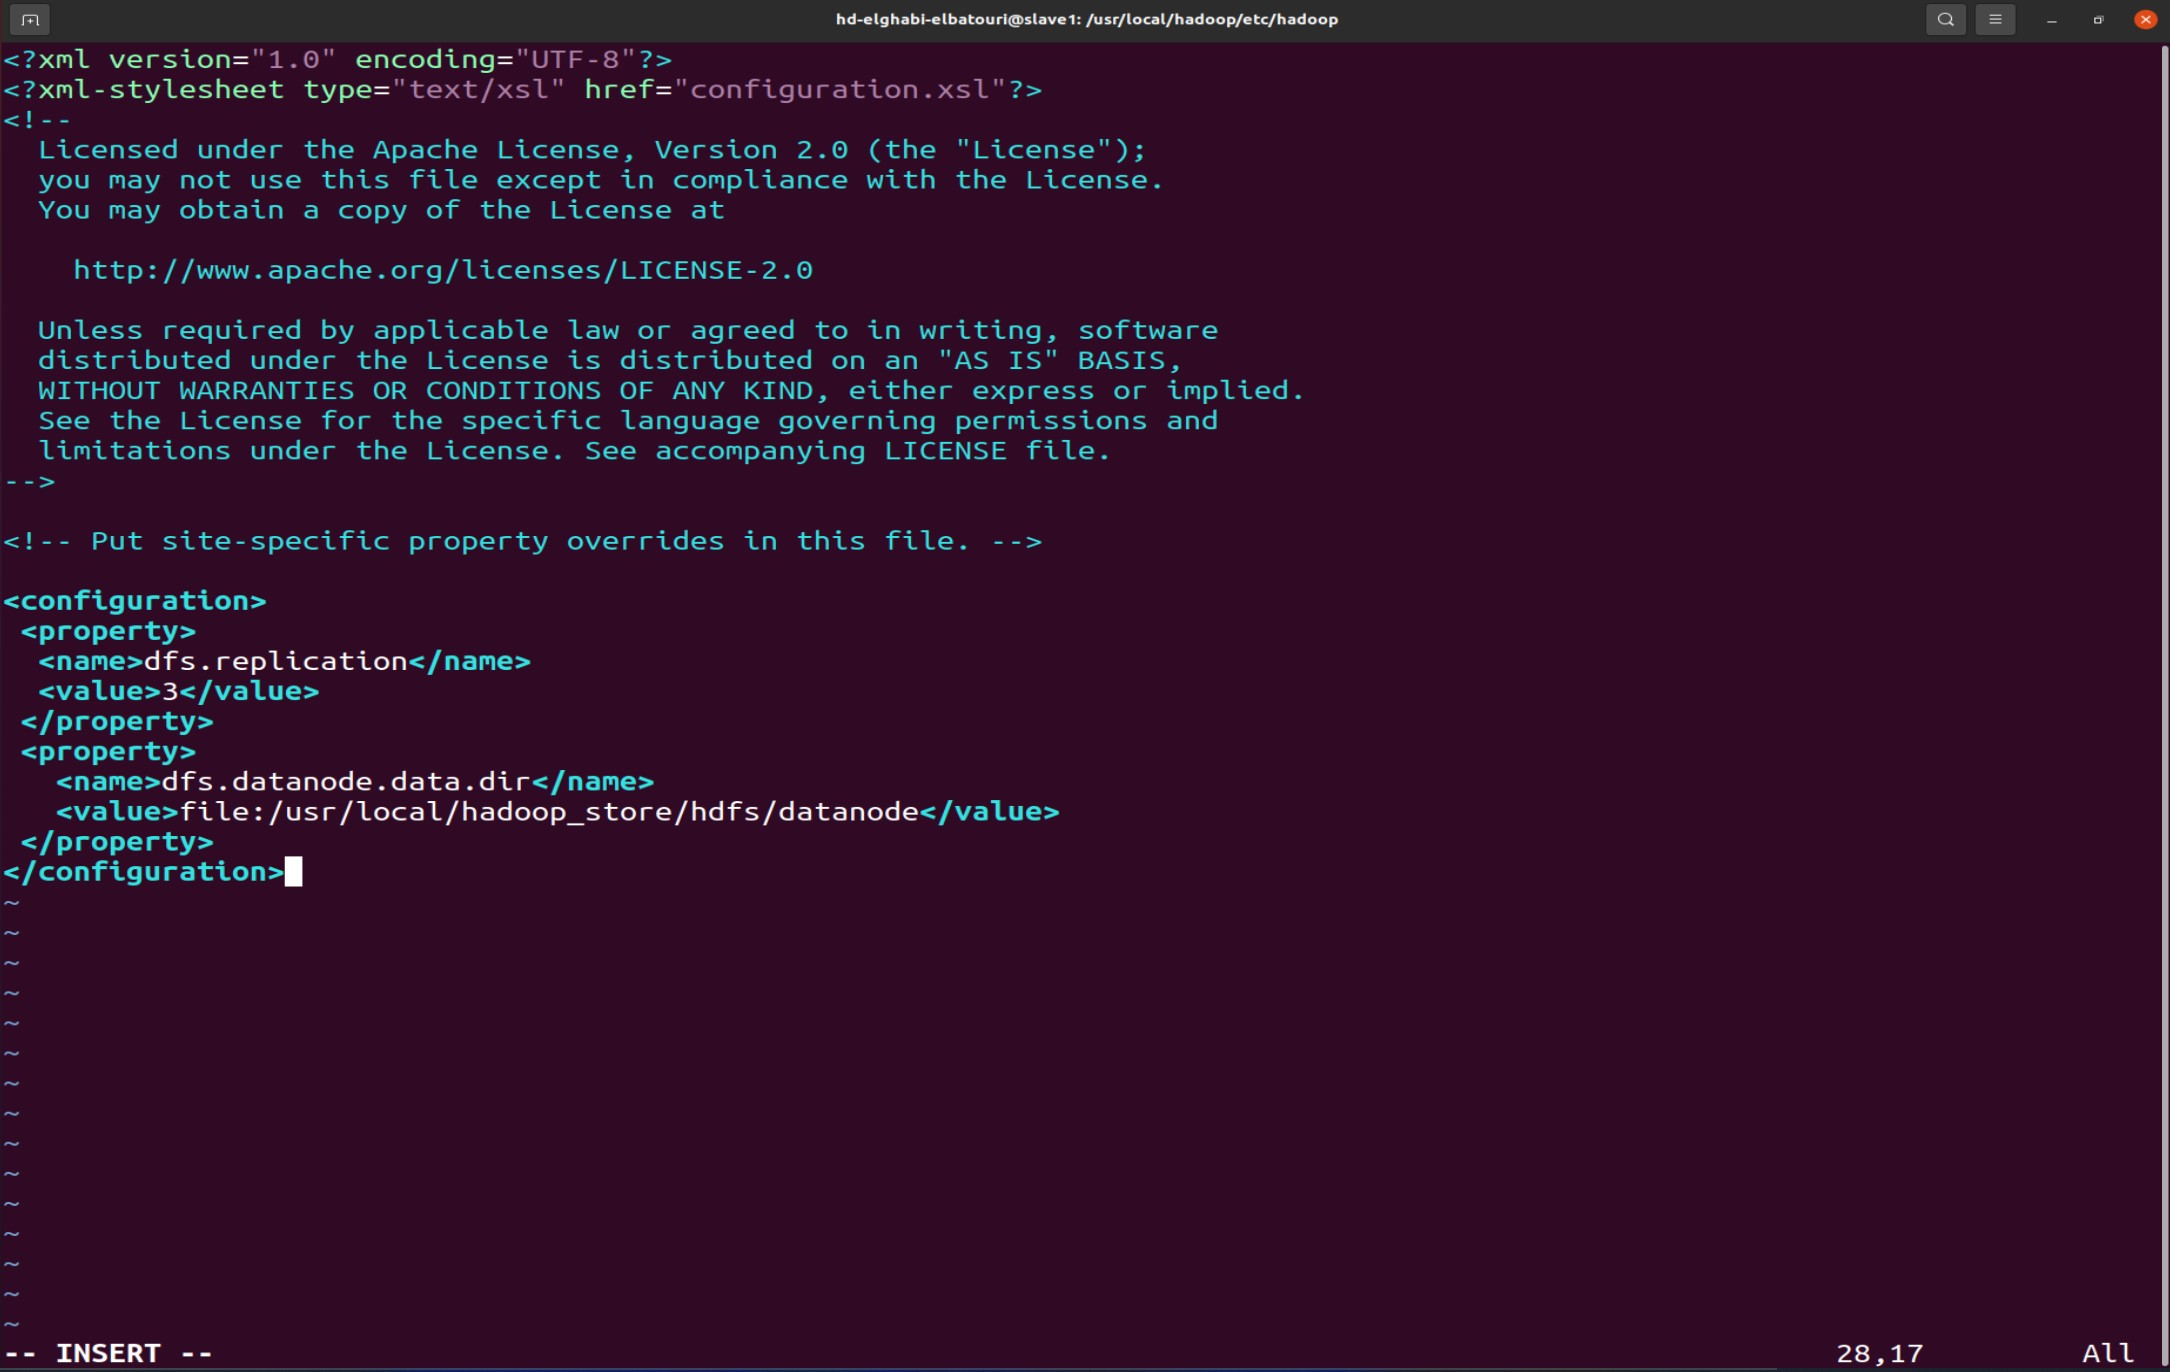
\includegraphics[width=1\linewidth]{Big_Data/Hadoop/Multi-Nodes Cluster/Changing replication number.jpg} 
\end{center} 
\caption{caption} 
\end{figure} 
\FloatBarrier

\par Modifying the slaves file for hadoopmaster, slave1 and slave2.
\\
\begin{figure}[!htb] 
\begin{center} 
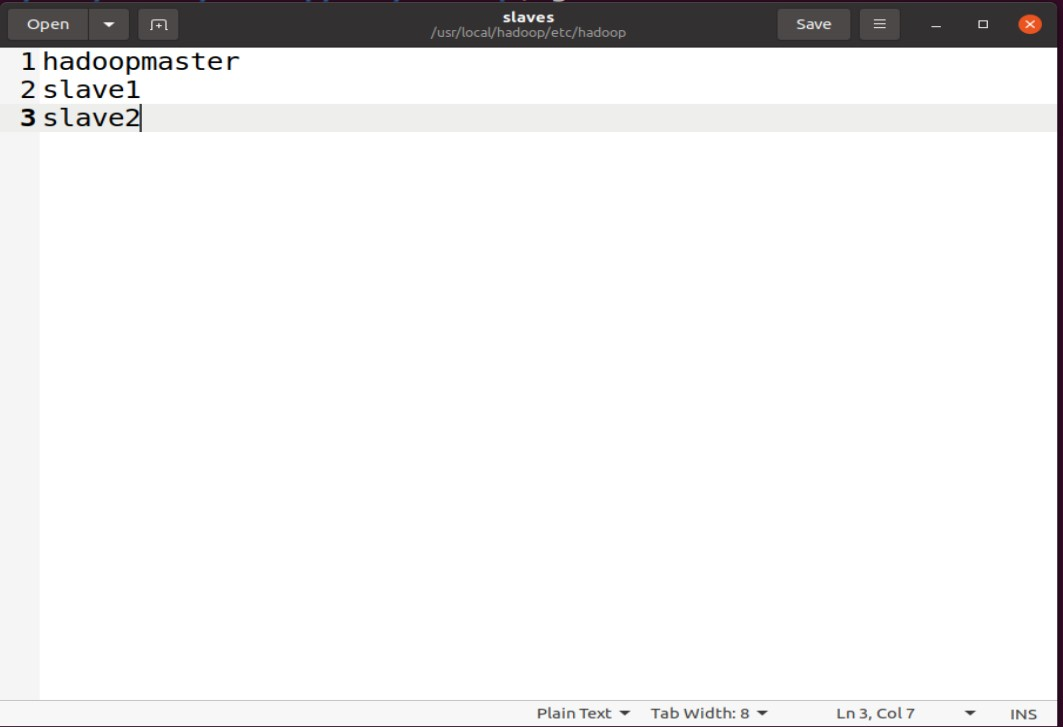
\includegraphics[width=1\linewidth]{Big_Data/Hadoop/Multi-Nodes Cluster/Editing slaves file.jpg} 
\end{center} 
\caption{caption} 
\end{figure} 
\FloatBarrier

\par Then empty the hadoop storage directory, and create the new directories.
\\
\begin{figure}[!htb] 
\begin{center} 
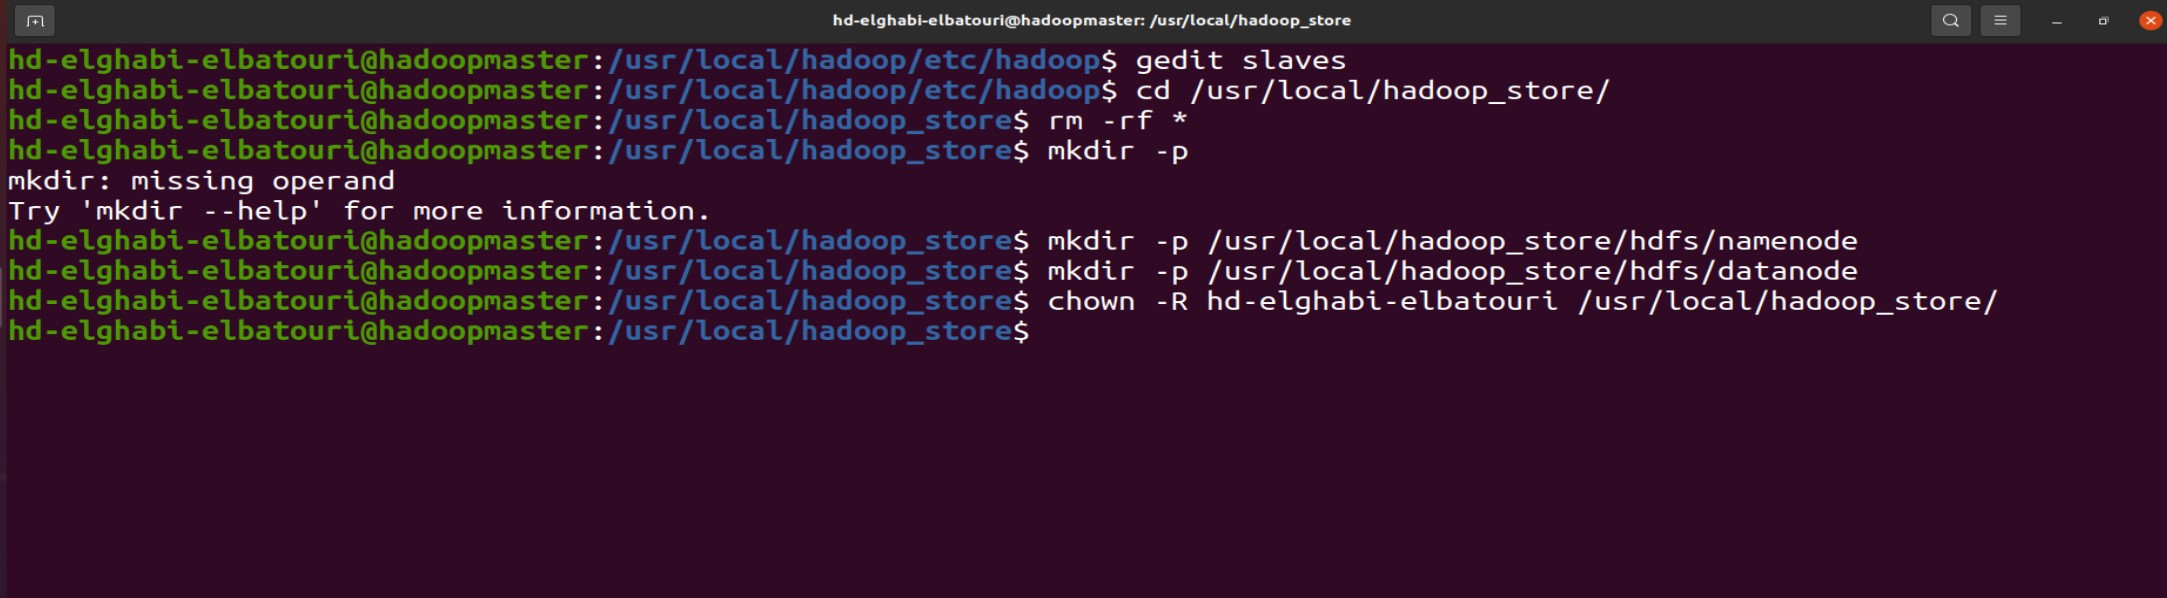
\includegraphics[width=1\linewidth]{Big_Data/Hadoop/Multi-Nodes Cluster/Creating new storage repo.jpg} 
\end{center} 
\caption{caption} 
\end{figure} 
\FloatBarrier
\end{spacing}